\chapter{问题的分解及分而治之算法}

\textbf{本章主要内容}

1.	第一个例子:归并排序
\begin{itemize}
    \item   用循环不变量的方法证明程序的正确性
	\item   递归算法的时间复杂度
\end{itemize}

2.	其他例子:逆序对计数,最近点对,乘法和快速傅里叶变换。

3.	分治算法和随机算法结合在一起有很好的应用:快速排序算法,选择数算法。
分治算法的优势:有些问题使用暴力破解算法已经是多项式时间复杂度,但使用分治算法使得复杂度还能降低。比如最近点对的算法复杂度。

\section{排序问题}
\subsection{算法策略}

如果一个问题可以分成更小的子问题,我们有以下2种策略:

(1) 增量式:一个数排序,增加一个数,2个数排序,直到n个数排序。

(2) 分治算法:大刀阔斧的分,n个问题分两半,n/2的问题不会,则再分成n/4,直到能解决为止。

\subsubsection{增量式策略}
	
	基本思想:假设我们有一个部分解,例如 A[0..j-1]已经被正确排序,将A[j]加入进来并放入正确的位置,那么A[0..j]就被排好序了。
	
	举例分析:插入排序。具体代码如下:
	
\noindent
\begin{small}
{\sc InsertionSort}( A ) 
\begin{algorithmic}[1]
\FOR{$j=0$ to $n-1$} 
\STATE $key = A[j];$ 
\STATE $i = j - 1;$
\WHILE{ $ i \geq 0$ and $A[i] > key $}
\STATE $A[i+1] = A[i];$ 
\STATE $i--;$
\ENDWHILE
\STATE $A[i+1] = key;$
\ENDFOR
\end{algorithmic}
\end{small}

\begin{itemize}

\item 最差的情况:数组是倒序排列的,那么每一个数加进来后,由于比前面所有的数都小,前面的数都要向后挪一个位置,因此$T(n)= 1+2+3+...+n$

\item 
插入排序的时间复杂度分析: $O(n^2)$. 

\item 迭代表达式表示为:$T(n) = T(n-1) + cn =
O(n^2)$.
\end{itemize}

\subsubsection{分治策略}

归并排序:第一次是被冯诺依曼在1940s提出的。

重要观察:一个问题能被划分成2个独立的子问题。具体步骤如下:

\begin{itemize}
\item Divide:将n个元素的序列分成2个分别有n/2个元素的序列

\item Conquer:假设每个子问题能被解决,实现方法是使用递归调用。

\item Merge:将2个排序好的子序列合并成一个序列,得到原始问题的解。
\end{itemize}

算法伪代码如下:

\noindent
\begin{small}

{\sc MergeSort}$( A, l, r )$
\begin{algorithmic}[1] 
\STATE/* To sort part of the array $A[l..r]$. */
\IF{ $ l < r$ }
	\STATE $m = ( l + r )/ 2; $ // $m$ denotes the middle point; 
	\STATE {\sc MergeSort}( A, l, m ); 
	\STATE {\sc MergeSort}( A,m, r); 
	\STATE {\sc Merge}(A, l, m, r); // combining the sorted subsequences; 
\ENDIF
\end{algorithmic}
\end{small}

	第4步和第5步是将数组A[l..r]分成A[l..m]和A[m..r],并对两个子问题递归调用求解。第6步将2个部分解合并成最终解。
	
	举例分析归并排序的具体做法
	
	(一)怎么分?

\begin{figure}[H]
\centering
    
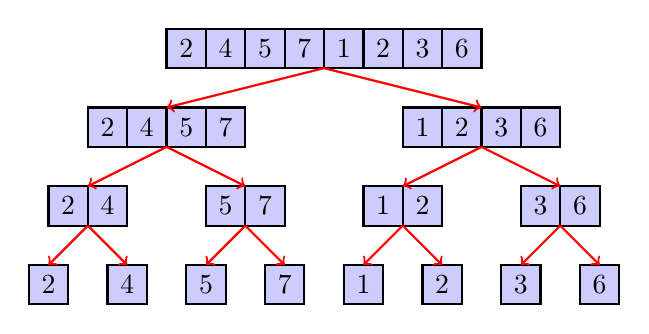
\begin{tikzpicture}
 
  \foreach \i/\name in { 0/2,1/4,2/5,3/7,4/1, 5/2, 6/3, 7/6 } {
         \draw[  fill=blue!20, thick ] (\i*0.5,0) rectangle (\i*0.5+0.5, 0.5);
         \node at (\i*0.5+0.25, 0.5/2) {$\name$};
 }
 
 %level 2
  
   \foreach \i/\name in { 0/2,1/4,2/5,3/7 } {
         \draw[  fill=blue!20, thick ] (\i*0.5-1,0-1) rectangle (\i*0.5-1+0.5, 0.5-1);
         \node at (\i*0.5+0.25-1, 0.5/2-1) {$\name$};
 }
 
    \foreach \i/\name in { 4/1, 5/2, 6/3, 7/6 } {
         \draw[  fill=blue!20, thick ] (\i*0.5+1,0-1) rectangle (\i*0.5+1+0.5, 0.5-1);
         \node at (\i*0.5+0.25+1, 0.5/2-1) {$\name$};
 }
  
  %level 3
     \foreach \i/\name in { 0/2,1/4 } {
         \draw[  fill=blue!20, thick ] (\i*0.5-1-0.5,0-2) rectangle (\i*0.5-1+0.5-0.5, 0.5-2);
         \node at (\i*0.5+0.25-1-0.5, 0.5/2-2) {$\name$};
 }
 
      \foreach \i/\name in { 2/5,3/7 } {
         \draw[  fill=blue!20, thick ] (\i*0.5-1+0.5,0-2) rectangle (\i*0.5-1+0.5+0.5, 0.5-2);
         \node at (\i*0.5+0.25-1+0.5, 0.5/2-2) {$\name$};
 }
 
     \foreach \i/\name in { 4/1, 5/2 } {
         \draw[  fill=blue!20, thick ] (\i*0.5+1-0.5,0-2) rectangle (\i*0.5+1+0.5-0.5, 0.5-2);
         \node at (\i*0.5+0.25+1-0.5, 0.5/2-2) {$\name$};
 }
 
      \foreach \i/\name in { 6/3, 7/6 } {
         \draw[  fill=blue!20, thick ] (\i*0.5+1+0.5,0-2) rectangle (\i*0.5+1+0.5+0.5, 0.5-2);
         \node at (\i*0.5+0.25+1+0.5, 0.5/2-2) {$\name$};
 }
 
 %level 4
      \foreach \i/\name in { 0/2 } {
         \draw[  fill=blue!20, thick ] (\i*0.5-1-0.5 -0.25,0-3) rectangle (\i*0.5-1+0.5-0.5 -0.25, 0.5-3);
         \node at (\i*0.5+0.25-1-0.5 -0.25, 0.5/2-3) {$\name$};
 }
 
       \foreach \i/\name in { 1/4 } {
         \draw[  fill=blue!20, thick ] (\i*0.5-1-0.5 +0.25,0-3) rectangle (\i*0.5-1+0.5-0.5 +0.25, 0.5-3);
         \node at (\i*0.5+0.25-1-0.5 + 0.25, 0.5/2-3) {$\name$};
 }
 
       \foreach \i/\name in { 2/5 } {
         \draw[  fill=blue!20, thick ] (\i*0.5 - 1 + 0.5 - 0.25,0-3) rectangle (\i*0.5 - 1 + 0.5 + 0.5 - 0.25, 0.5-3);
         \node at (\i*0.5+0.25-1 + 0.5 - 0.25, 0.5/2-3) {$\name$};
 }
 
        \foreach \i/\name in { 3/7 } {
         \draw[  fill=blue!20, thick ] (\i*0.5 - 1 + 0.5 + 0.25,0-3) rectangle (\i*0.5 - 1 + 0.5 + 0.5 + 0.25, 0.5-3);
         \node at (\i*0.5+0.25-1 + 0.5 + 0.25, 0.5/2-3) {$\name$};
 }


     \foreach \i/\name in { 4/1 } {
         \draw[  fill=blue!20, thick ] (\i*0.5+1-0.5 - 0.25 ,0-3) rectangle (\i*0.5+1+0.5-0.5 - 0.25, 0.5-3);
         \node at (\i*0.5+0.25+1-0.5 -0.25, 0.5/2-3) {$\name$};
 }
 
      \foreach \i/\name in {  5/2 } {
         \draw[  fill=blue!20, thick ] (\i*0.5+1-0.5 + 0.25 ,0-3) rectangle (\i*0.5+1+0.5-0.5+ 0.25, 0.5-3);
         \node at (\i*0.5+0.25+1-0.5+ 0.25, 0.5/2-3) {$\name$};
 }
 
      \foreach \i/\name in { 6/3 } {
         \draw[  fill=blue!20, thick ] (\i*0.5+1+0.5 - 0.25,0-3) rectangle (\i*0.5+1+0.5+0.5 - 0.25, 0.5-3);
         \node at (\i*0.5+0.25+1+0.5 - 0.25, 0.5/2-3) {$\name$};
 }
 
      \foreach \i/\name in { 7/6 } {
         \draw[  fill=blue!20, thick ] (\i*0.5+1+0.5 + 0.25,0-3) rectangle (\i*0.5+1+0.5+0.5 + 0.25, 0.5-3);
         \node at (\i*0.5+0.25+1+0.5 + 0.25, 0.5/2-3) {$\name$};
 }
 
 % lines 
 \foreach \source/\dest in {{( 4*0.5 , 0)/( 2*0.5 - 1, -0.5)}, {( 4*0.5 , 0)/( 6*0.5 + 1, -0.5)}} 
 	\path[draw=red, ->, thick]  \source  --  \dest;
 
  \foreach \source/\dest in {{( 2*0.5 - 1, -1)/( 1*0.5 - 1 -0.5, -1.5)}, {( 2*0.5 - 1, -1)/( 3*0.5 - 1 +0.5, -1.5)},{( 6*0.5 + 1, -1)/( 5*0.5 + 1 - 0.5, -1.5)},{( 6*0.5 + 1, -1)/( 7*0.5 + 1 + 0.5, -1.5)}} 
 	\path[draw=red, ->, thick]  \source  --  \dest;
  
    \foreach \source/\dest in {{( 1*0.5 - 1 -0.5, -2)/( 1*0.5 - 1 -0.5 - 0.5, -2.5)}, {( 1*0.5 - 1 -0.5, -2)/( 1*0.5 - 1 -0.5 + 0.5, -2.5)}, {( 3*0.5 - 1 +0.5, -2)/( 3*0.5 - 1 +0.5 + 0.5, -2.5)},{( 3*0.5 - 1 +0.5, -2)/( 3*0.5 - 1 +0.5 - 0.5, -2.5)}, {( 5*0.5 + 1 - 0.5, -2)/( 5*0.5 + 1 - 0.5 + 0.5, -2.5)},{( 5*0.5 + 1 - 0.5, -2)/( 5*0.5 + 1 - 0.5 - 0.5, -2.5)}, {( 7*0.5 + 1 + 0.5, -2)/( 7*0.5 + 1 + 0.5 + 0.5, -2.5)},{( 7*0.5 + 1 + 0.5, -2)/( 7*0.5 + 1 + 0.5 - 0.5, -2.5)}} 
 	\path[draw=red, ->, thick]  \source  --  \dest;
	
  
\end{tikzpicture}

\end{figure}

	对于不会解的问题,将其分解到能被解决为止,在这里2个数的比较是算法的基础解,能被解决。
	
	(二)怎么合并?
	合并算法如下所示:
	
\noindent
{\sc Merge} $( A, l, m, r )$
\begin{footnotesize}
\begin{algorithmic}[1]
\STATE /* to merge $A[l..m]$(named as $L$) and $A[m+1..r]$ (named as $R$). */
\STATE $i=0;$ $j=0;$
\FOR { $k = l $ to $r$ }
\IF{ $L[i] < R[j]$ }
\STATE $A[k] = L[i];$
\STATE $i++;$
\ELSE
\STATE $A[k] = R[j];$
\STATE $j++;$
\ENDIF
\ENDFOR
\end{algorithmic}
\end{footnotesize}
	
\begin{figure}[H]
\centering
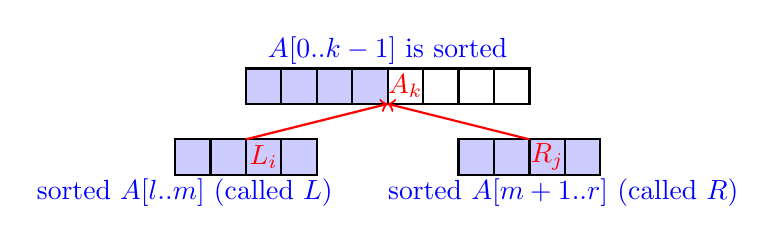
\begin{tikzpicture}[scale=0.9, auto,swap]
 
  \foreach \i/\name in { 0/,1/,2/,3/ } {
         \draw[  fill=blue!20, thick ] (\i*0.5,0) rectangle (\i*0.5+0.5, 0.5);
         \node at (\i*0.5+0.25, 0.5/2) {$\name$};
 }
 
  \foreach \i/\name in { 4/A_k, 5/, 6/, 7/ } {
         \draw[   thick ] (\i*0.5,0) rectangle (\i*0.5+0.5, 0.5);
         \node[red] at (\i*0.5+0.25, 0.5/2) {$\name$};
 }
 

 %level 2
  
   \foreach \i/\name in { 0/,1/,2/L_i,3/ } {
         \draw[  fill=blue!20, thick ] (\i*0.5-1,0-1) rectangle (\i*0.5-1+0.5, 0.5-1);
         \node[red] at (\i*0.5+0.25-1, 0.5/2-1) {$\name$};
 }
 
    \foreach \i/\name in { 4/, 5/, 6/R_j, 7/} {
         \draw[  fill=blue!20, thick ] (\i*0.5+1,0-1) rectangle (\i*0.5+1+0.5, 0.5-1);
         \node[red] at (\i*0.5+0.25+1, 0.5/2-1) {$\name$};
 }
  

 % lines 
 \foreach \source/\dest in {{( 4*0.5 , 0)/( 2*0.5 - 1, -0.5)}, {( 4*0.5 , 0)/( 6*0.5 + 1, -0.5)}} 
 	\path[draw=red, <-, thick]  \source  --  \dest;
 
\node[blue] at (2, 0.5/2-1.5) {sorted $A[l..m]$ (called $L$)\qquad sorted $A[m+1..r]$ (called $R$)};
\node[blue] at (2, 0.75) { $A[0..k-1]$ is sorted};
    
\end{tikzpicture}
\end{figure}

	左边一半存入数组L和右边一半存入数组R都是已经排好的子序列,如何将2者合并成一个序列呢?
	
	每次取两个数组最小的元素,取2者最小的填入数组A中,然后将数组下标右移一位。

	a)	证明merge策略的正确性:循环不变量技术
\begin{itemize}

\item 循环不变量:类似于数学归纳法技术。

\item 初始情况:$k=l$.因为A[l..k-1]为空,所以循环不变量成立。

\item 特征保持:假设$L[i]<R[j]$,而且A[l..k-1]有k-l个最小的数,那么把L[i]放到A[k],A[l..k]就是拥有k-l+1个最小的数
\end{itemize}
	b)	Merge算法的时间复杂度
	
	For循环最多执行n次,故时间复杂度是$O(n)$。

	(三)	归并排序的时间复杂度
	
	假设T(n)是整个问题的时间复杂度,将其分成2半,左边需要$T(n/2)$,右边需要$T(n/2)$,那么可以写成如下:
	
\begin{equation}
T(n) = \begin{cases}
         c & n = 2 \\ T(n/2) + T(n/2) + cn  & otherwise
        \end{cases}
\end{equation}

\begin{figure}[H]
\centering
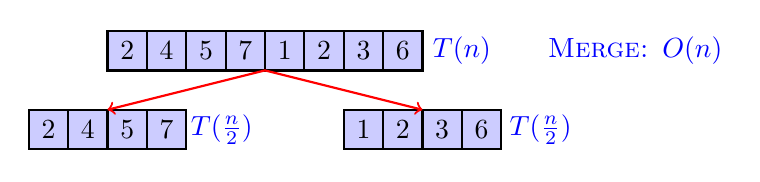
\begin{tikzpicture}[scale=1., auto,swap]
 
  \foreach \i/\name in { 0/2,1/4,2/5,3/7,4/1, 5/2, 6/3, 7/6 } {
         \draw[  fill=blue!20, thick ] (\i*0.5,0) rectangle (\i*0.5+0.5, 0.5);
         \node at (\i*0.5+0.25, 0.5/2) {$\name$};
 }
 
 \node[blue] at (8*0.5 + 0.5, 0.5/2) {$T(n)$};
  \node[blue] at (8*0.5 + 2.7, 0.5/2) {{\sc Merge: }$O(n)$};
 \node[blue] at (4*0.5-0.55 , 0.5/2-1) {$T(\frac{n}{2})$};
 \node[blue] at (8*0.5 + 1.5, 0.5/2-1) {$T(\frac{n}{2})$};
 
 %level 2
  
   \foreach \i/\name in { 0/2,1/4,2/5,3/7 } {
         \draw[  fill=blue!20, thick ] (\i*0.5-1,0-1) rectangle (\i*0.5-1+0.5, 0.5-1);
         \node at (\i*0.5+0.25-1, 0.5/2-1) {$\name$};
 }
 
    \foreach \i/\name in { 4/1, 5/2, 6/3, 7/6 } {
         \draw[  fill=blue!20, thick ] (\i*0.5+1,0-1) rectangle (\i*0.5+1+0.5, 0.5-1);
         \node at (\i*0.5+0.25+1, 0.5/2-1) {$\name$};
 }
  
  
 % lines 
 \foreach \source/\dest in {{( 4*0.5 , 0)/( 2*0.5 - 1, -0.5)}, {( 4*0.5 , 0)/( 6*0.5 + 1, -0.5)}} 
 	\path[draw=red, ->, thick]  \source  --  \dest;
 
	
  
\end{tikzpicture}

\end{figure}

	从插入排序到归并排序,复杂度从$O(n^2)$到$O(n\log n)$,那么节省的究竟是什么呢?
	
	下图表示的箭头数量是2种算法排序过程中需要进行的比较次数。
	
\begin{figure}[H]
  \begin{minipage}{0.45\textwidth} 
  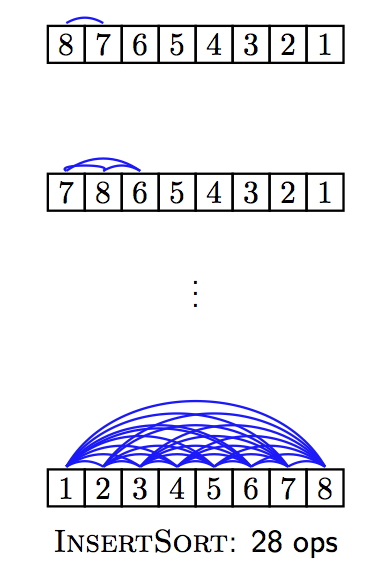
\includegraphics[height=2.7in] {L5-insertsort-left.png}
 \end{minipage}
  \begin{minipage}{0.45\textwidth} 
 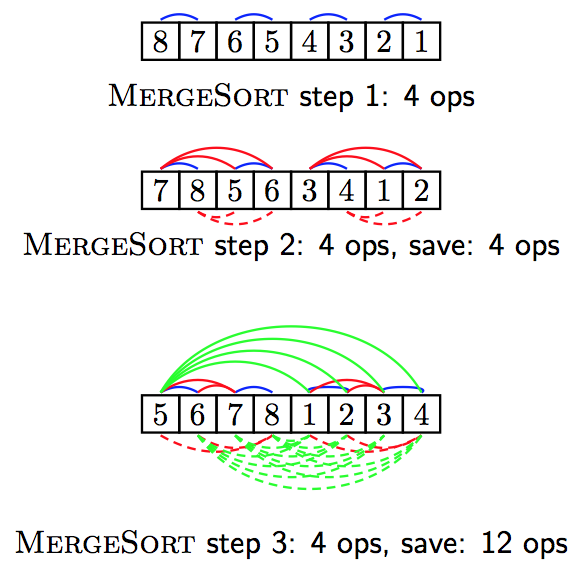
\includegraphics[height=2.75in] {L5-mergesort-right.png}
 \end{minipage}
\end{figure}
	我们可以看出,插入排序需要28次比较。而归并排序中第2步省去了4次比较,第3步省去了12次比较。例如:第3步中,5和7比较之后,不需要再和8进行比较。
	
\subsubsection{分治算法的复杂度}

	归并排序的时间复杂度:如何精确计算分治算法的时间复杂度?
	
	我们已经得到算法复杂度的递归表达式,如何将递归表达式写成精确地结果?主要有以下3种方法。
\begin{itemize}

\item 将表达式展开,展开一定程度之后就会观察到结果的模型。

\item 猜测并证明猜测的正确性。

\item 产生函数
\end{itemize}

	本书只讲前2种方法。
\newpage

\noindent
(1)复杂度分析方法--展开
\begin{itemize}
\item 
将$T(n)$分成$T(n/2)$的表达式,如果还看不出结果的话继续展开。

\begin{figure}[H]
\centering
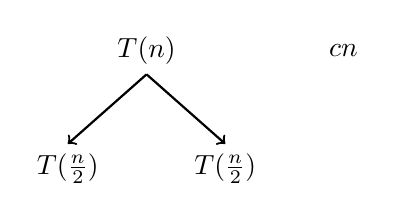
\begin{tikzpicture}[scale=1., auto,swap]
 %l1
 \node[ ] (l1) at (0,0) {$T(n)$};
 
 
 %l2
 \node[ ] (l21) at (-1,-1.5) {$T(\frac{n}{2})$};
 \node[ ] (l22) at (1,-1.5) {$T(\frac{n}{2})$};
  
 %lines
 \path[draw, ->, thick] (l1.south) -- (l21.north); 
  \path[draw, ->, thick] (l1.south) -- (l22.north);
   
      
      %cn
      \node[ ] (l1) at (2.5,0) {$\hdots cn$};  

      
\end{tikzpicture}
\end{figure}
\item
如果还不能解决,将$T(n/2)$的问题展开成 $T(n/4)$的问题,直到能被解决为止。

\begin{figure}[H]

\centering

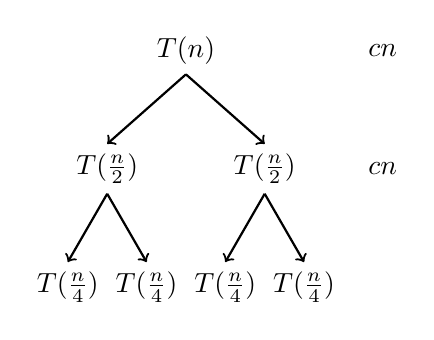
\begin{tikzpicture}[scale=1., auto,swap]
 %l1
 \node[ ] (l1) at (0,0) {$T(n)$};
 
 
 %l2
 \node[ ] (l21) at (-1,-1.5) {$T(\frac{n}{2})$};
 \node[ ] (l22) at (1,-1.5) {$T(\frac{n}{2})$};
 %l3
 \node[ ] (l31) at (-1 - 0.5,-3) {$T(\frac{n}{4})$};
 \node[ ] (l32) at (-1 + 0.5,-3) {$T(\frac{n}{4})$};
 
  \node[ ] (l33) at (1 - 0.5,-3) {$T(\frac{n}{4})$};
 \node[ ] (l34) at (1 + 0.5,-3) {$T(\frac{n}{4})$};
 
 %lines
 \path[draw, ->, thick] (l1.south) -- (l21.north); 
  \path[draw, ->, thick] (l1.south) -- (l22.north);
   
 \path[draw, ->, thick] (l21.south) -- (l31.north); 
 \path[draw, ->, thick] (l21.south) -- (l32.north); 

 \path[draw, ->, thick] (l22.south) -- (l33.north); 
 \path[draw, ->, thick] (l22.south) -- (l34.north); 
      
      %cn
      \node[ ] (l1) at (2.5,0) {$\hdots cn$};  
      \node[ ] (l1) at (2.5,-1.5) {$\hdots cn$}; 
 
\end{tikzpicture}
\end{figure}

\item 
直到展开的子问题的时间是常数。那么我们只需要计算最后一层常数时间的子问题的个数。
\begin{figure}[H]

\centering
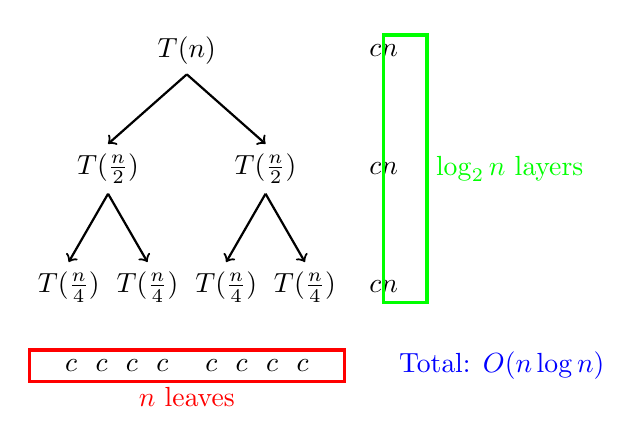
\begin{tikzpicture}[scale=1., auto,swap]
 %l1
 \node[ ] (l1) at (0,0) {$T(n)$};
 
 
 %l2
 \node[ ] (l21) at (-1,-1.5) {$T(\frac{n}{2})$};
 \node[ ] (l22) at (1,-1.5) {$T(\frac{n}{2})$};
 %l3
 \node[ ] (l31) at (-1 - 0.5,-3) {$T(\frac{n}{4})$};
 \node[ ] (l32) at (-1 + 0.5,-3) {$T(\frac{n}{4})$};
 
  \node[ ] (l33) at (1 - 0.5,-3) {$T(\frac{n}{4})$};
 \node[ ] (l34) at (1 + 0.5,-3) {$T(\frac{n}{4})$};
 
 %lines
 \path[draw, ->, thick] (l1.south) -- (l21.north); 
  \path[draw, ->, thick] (l1.south) -- (l22.north);
   
 \path[draw, ->, thick] (l21.south) -- (l31.north); 
 \path[draw, ->, thick] (l21.south) -- (l32.north); 

 \path[draw, ->, thick] (l22.south) -- (l33.north); 
 \path[draw, ->, thick] (l22.south) -- (l34.north); 
      
      %cn
      \node[ ] (l1) at (2.5,0) {$\hdots cn$};  
      \node[ ] (l1) at (2.5,-1.5) {$\hdots cn$}; 
      \node[ ] (l1) at (2.5,-3) {$\hdots cn$}; 

     \node[ ] (l1) at (0,-3.5) {$\hdots \hdots \hdots \hdots $}; 

     \node[ ] (l1) at (0,-4) {$c\ \ c\ \ c\ \ c\ \ \ \ c\ \ c\ \ c\ \ c$}; 
      

      %boxes
      \draw[ green, very thick ]  (2.5, 0.2) rectangle (3.05, -3.2);
      \draw[ red, very thick ] (-2, -4.2) rectangle (2, -3.8);

%total      
         \node[ red ] (l1) at (0,-4.4) {$n$ leaves}; 
          \node[ green ] (l1) at (4.1,-1.5) {$\log_2 n$ layers}; 
	\node[blue] at (4.0, -4.0) {Total: $O(n\log n)$ };

      
\end{tikzpicture}
\end{figure}

\end{itemize}

那么时间复杂度就由2部分组成:合并的时间和最后一层比较要花的时间。

那么究竟有多少层呢,很显然要层数是$O(\log_2 n)$。那么合并花的时间就是$cn*\log_{2} n$。
可以看出这棵树总共有n个叶子节点,花费时间是cn。

因此时间复杂度是$O(n\log n)$

(二)复杂度分析方法2--先猜测后证明

\begin{itemize}
 \item 
猜测一个解决方案并替换掉设定的系数,证明公式的正确性。
\item 
猜测: $T(n) \leq cn \log_2 n$ for all $n\geq 2$;
\item 
证明:  

\begin{itemize}
 \item 当 $n=2$: $T(2) = c \leq cn \log_2 n$; 
 \item 当 $n>2$: 假设对所有 $m\leq n$都有$T(m) \leq cm \log_2 m$ 。那么 \\ 
\begin{eqnarray}
T(n) &=&  2T(n/2) + cn \\
     &\leq&  2c(n/2)\log_2(n/2) + cn \\
     &=&  2c(n/2) \log_2 n - 2c(n/2) + cn\\
     &=& cn \log_2 n 
\end{eqnarray}
\end{itemize}
\end{itemize}


	但事实上,我们经常猜的没有那么准,我们可能只猜到 $T(n)= O(n\log n)$,或者写成$T(n)=k \log_b n$。K和b我们不清楚,再去求解。
	
	所以我们可能会猜测一个比较模糊的表达式,如下:
\begin{itemize}
 \item 
猜测和替换,我们只能猜测k和b可以等于多少,然后去替换掉。
\item 
模糊猜测: $T(n)=O(n\log n)$。时间复杂度这样描述 $T(n)=k \log_b n$,  \textcolor{red}{\bf $k,b$ 是待定系数}
\end{itemize}

\begin{eqnarray}
T(n) &=&  2 T(n/2) + cn  \nonumber \\
     &\leq&  2k(n/2)\log_b(n/2) + cn  \quad \text{(set b=2 for simplification)} \nonumber\\
     &=&  2k(n/2) \log_2 n - 2k(n/2) + cn \nonumber  \\
     &=& kn \log_2 n - kn + cn \quad \text{(set k=c for simplification again)}
     \nonumber \\ &=& c n \log_2 n  \quad \nonumber  
\end{eqnarray} 

\newpage

后来,大家把递归表达式总结成一个定理。定理描述如下:

假设 $T(n)$ 定义为$T(n)=aT(n/b) + f(n)$, 那么 $T(n)$ 会有如下性质: 
\begin{enumerate}
 \item If $f(n)=O(n^{\log_b a - \epsilon})$, then $T(n)=\Theta(n^{\log_b a })$;
 \item If $f(n)=\Theta(n^{\log_b a})$, then $T(n)=\Theta(n^{\log_b a }) \log n $;
 \item If $f(n)=\Omega(n^{\log_b a + \epsilon})$ and $a f(n/b) \leq c f(n)$, then $T(n)=\Theta( f(n) )$. Here, $\epsilon$ denotes a small, positive number. 
\end{enumerate}

举例分析如下
\begin{itemize}
 \item 
Example 1: $T(n) \leq 3 T(n/2) + cn$ (see a figure)
\ \\
$T(n) = O(n^{\log_2 3}) = O(n^{1.585})$


\ \\

\item 
Example 2: $T(n) \leq 2 T(\frac{n}{2}) + cn^2$ (see  a figure)

\ \\
$T(n)= \sum_{j=0}^{\log n} \frac{cn^2}{2^j}  = cn^2 \sum_{j=0}^{\log n} \frac{1}{2^j} = 2cn^2$

(Note: not $O(n^2 \log n)$ )


\ \\
\item 
Example 3: $T(n) \leq T(n/3) + T(2n/3) + cn$ (see a figure )
\end{itemize}



\section{逆序数计数问题}

\subsection{实际应用}
\begin{enumerate}
\item
识别2个人的相似度,比如比较2人对书本,电影等的排序。
\item
meta search engine, 它把搜索请求提交给其他搜索引擎,比较各个搜索引擎的排序结果,计算它们的相似度。
\end{enumerate}

逆序数问题的形式化表示
\begin{itemize}
 \item 
 输入:一组n个不同的数的序列
 \item
 输出:逆序对数,如果$i<j$,而$a_i>a_j$,那么就是逆序数对。
\end{itemize}

\begin{figure}[H]
\centering
 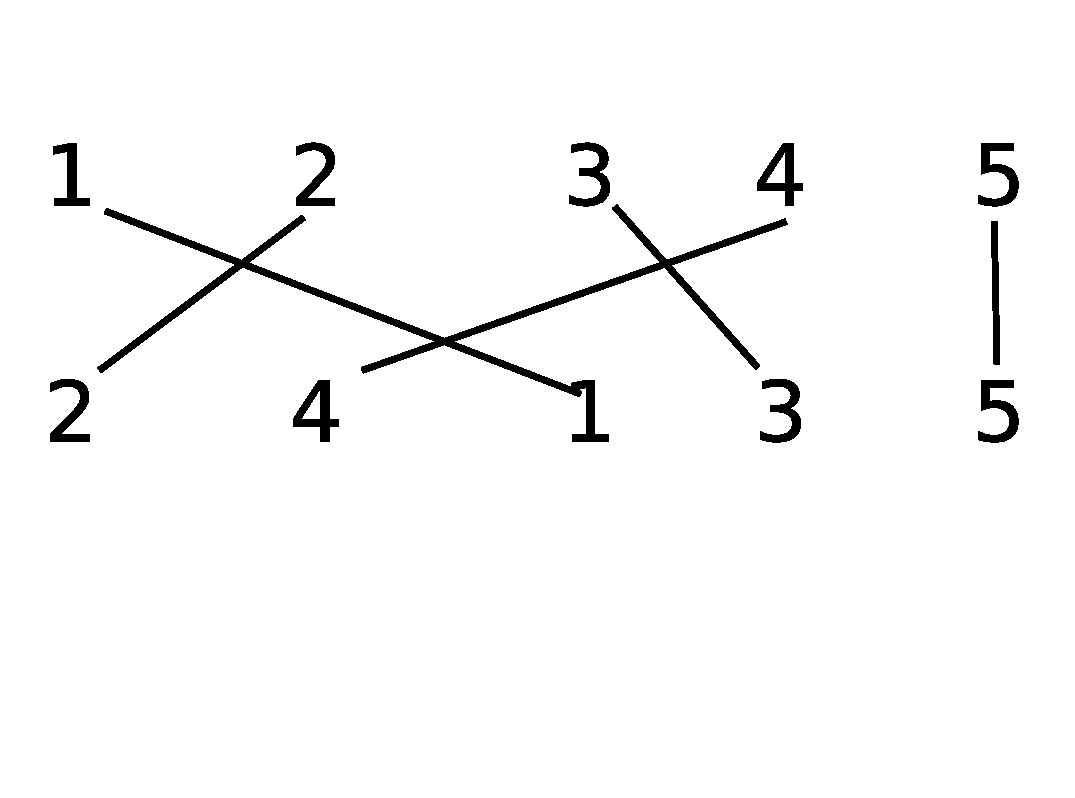
\includegraphics[width=2in] {L5-counting-inversion.eps}
\end{figure}

	如上图表示,将正确的排好的序列{1,2,3,4,5}和序列{2,4,1,3,5}相同的数连起来,那么连线交叉的数量就是逆序数的对数。比如1和2,1和4,3和4总共3对。


\subsubsection{逆序数的具体应用}
\begin{itemize}
\item
基因序列的比较
\begin{figure}[H]
\centering
 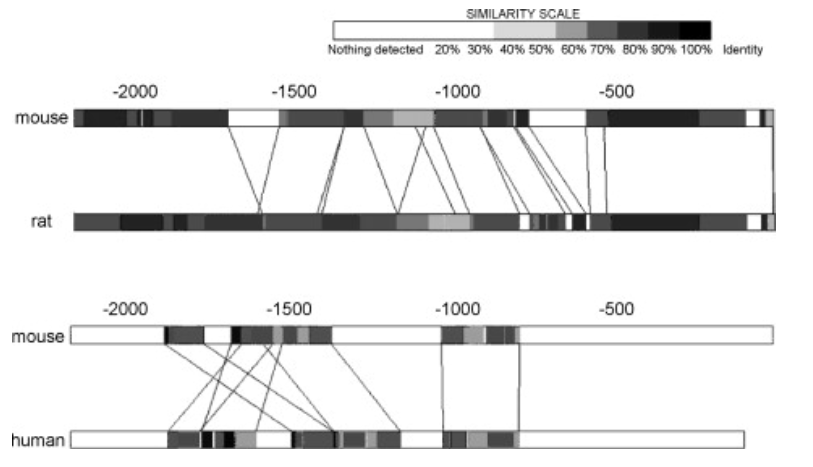
\includegraphics[width=3in] {L5-genome-comparison.png}
 \caption{Sequence comparison of the 5' flanking regions of mouse, rat and human ER$\beta$. } 
\end{figure}
	在生物信息领域,比较2个基因组是否一样,基因组有很多基因的排序,假设有n个基因,上图是mouse和rat之间基因序列的比较,相同的基因连成一条线,交叉的地方就是逆序。老鼠和人的基因的相似情况同样如此。
	
\item
求2个数列的相似度

常用方法:1.Pearson系数。2.Spearman相关系数。
新的策略: 
\begin{center} 
			 $W_1 = \sum_{i=1}^{n-k+1} (I_i^+, I_i^-)$ 
			 \end{center}
\end{itemize}
	表达式的含义是求相同长度子序列的相似度。举例分析
	\begin{center} 
$	X:\ 1\ 3\ 4\ 2\ 5$\\

$	Y:\ 1\ 4\ 5\ 2\ 3$
\end{center}
		
	$W_1 = 2$ when $k=3$.当设定比对的序列长度(滑动窗口)是3时,(1,3,4)和(1,4,5)是没有逆序的,(3,4,2)和(4,5,2)是没有逆序的,(4,2,5)和(5,2,3)是有逆序的。那么相似度就是2。这种算法的结果比Pearson系数要好。
	
	求逆序数的算法:暴力方法:枚举所有的点对,然后得到逆序数的结果,时间复杂度是$O(n^{2})$。那么有改善的算法吗?
\subsection{分治策略}


重要观察:逆序数问题能够被划分成几个子问题。 

分治策略: 
\begin{enumerate}
 \item  Divide: 分成2个序列: $A[0..n/2]$ 和 $A[n/2+1...n-1]$;
 \item Conquer: 递归调用计算各一半的逆序数;
 \item Combine:怎么比较分别位于左边和右边的数呢?
% \item \textcolor{blue}{\bf Combine:} how to count inversion ($a_i$,$a_j$), when \textcolor{red}{ $a_i$ and $a_j$ are in different half?} \\
%       We will get a $O(n\log n)$ algorithm if we can perform {\bf combine} step in $O(n)$ time. 
\end{enumerate}


\begin{figure}[H]
\centering
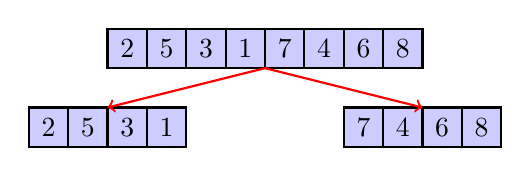
\begin{tikzpicture}[scale=1., auto,swap]
 
  \foreach \i/\name in { 0/2,1/5,2/3,3/1,4/7, 5/4, 6/6, 7/8 } {
         \draw[  fill=blue!20, thick ] (\i*0.5,0) rectangle (\i*0.5+0.5, 0.5);
         \node at (\i*0.5+0.25, 0.5/2) {$\name$};
 }
 

 %level 2
  
   \foreach \i/\name\n in { 0/2/s2,1/5/s5,2/3/s5,3/1/s1 } {
         \draw[  fill=blue!20, thick ] (\i*0.5-1,0-1) rectangle (\i*0.5-1+0.5, 0.5-1);
         \node (\n) at (\i*0.5+0.25-1, 0.5/2-1) {$\name$};
 }
 
    \foreach \i/\name/\n in { 4/7/s7, 5/4/s4, 6/6/s6, 7/8/s8 } {
         \draw[  fill=blue!20, thick ] (\i*0.5+1,0-1) rectangle (\i*0.5+1+0.5, 0.5-1);
         \node (\n) at (\i*0.5+0.25+1, 0.5/2-1) {$\name$};
 }
 
  
 % lines 
 \foreach \source/\dest in {{( 4*0.5 , 0)/( 2*0.5 - 1, -0.5)}, {( 4*0.5 , 0)/( 6*0.5 + 1, -0.5)}} 
 	\path[draw=red, ->, thick]  \source  --  \dest;
 
	
\end{tikzpicture}
\end{figure}

(一)合并策略1

	简单的枚举算法的话,需要$\frac{n^2}{4}$ 次比较。因此$T(n) = 2T(\frac{n}{2})  + \frac{n^2}{4} = O(n^2)$. 

	对于通用的分治算法的递归表达式$T(n) = aT(\frac{n}{b})  + f(n)$,由于这里的合并时间消耗$f(n)=\frac{n^2}{4} $,所以时间复杂度太大。


\begin{figure}[H]
\centering
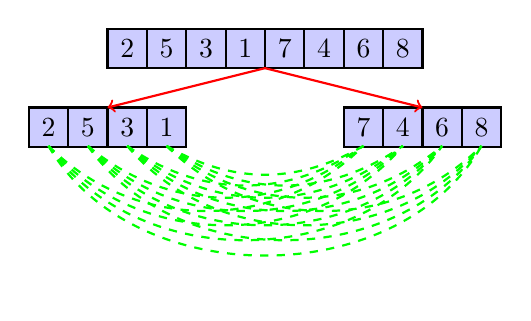
\begin{tikzpicture}[scale=1., auto,swap]
 
  \foreach \i/\name in { 0/2,1/5,2/3,3/1,4/7, 5/4, 6/6, 7/8 } {
         \draw[  fill=blue!20, thick ] (\i*0.5,0) rectangle (\i*0.5+0.5, 0.5);
         \node at (\i*0.5+0.25, 0.5/2) {$\name$};
 }

 %level 2
  
   \foreach \i/\name/\n in { 0/2/s2,1/5/s5,2/3/s3,3/1/s1} {
         \draw[  fill=blue!20, thick ] (\i*0.5-1,0-1) rectangle (\i*0.5-1+0.5, 0.5-1);
         \node (\n) at (\i*0.5+0.25-1, 0.5/2-1) {$\name$};
 }
 
    \foreach \i/\name/\n in { 4/7/s7, 5/4/s4, 6/6/s6, 7/8/s8} {
         \draw[  fill=blue!20, thick ] (\i*0.5+1,0-1) rectangle (\i*0.5+1+0.5, 0.5-1);
         \node (\n) at (\i*0.5+0.25+1, 0.5/2-1) {$\name$};
 }
 
  
 % lines 
 \foreach \source/\dest in {{( 4*0.5 , 0)/( 2*0.5 - 1, -0.5)}, {( 4*0.5 , 0)/( 6*0.5 + 1, -0.5)}} 
 	\path[draw=red, ->, thick]  \source  --  \dest;
 
\draw[green, dashed, thick] (s1.south) to [out=-30, in=180+30] (s7.south);
\draw[green, dashed, thick] (s1.south) to [out=-35, in=180+35] (s4.south);
\draw[green, dashed, thick] (s1.south) to [out=-40, in=180+40] (s6.south);
\draw[green, dashed, thick] (s1.south) to [out=-45, in=180+45] (s8.south);

\draw[green, dashed, thick] (s3.south) to [out=-35, in=180+35] (s7.south);
\draw[green, dashed, thick] (s3.south) to [out=-40, in=180+40] (s4.south);
\draw[green, dashed, thick] (s3.south) to [out=-45, in=180+45] (s6.south);
\draw[green, dashed, thick] (s3.south) to [out=-50, in=180+50] (s8.south);

\draw[green, dashed, thick] (s5.south) to [out=-40, in=180+40] (s7.south);
\draw[green, dashed, thick] (s5.south) to [out=-45, in=180+45] (s4.south);
\draw[green, dashed, thick] (s5.south) to [out=-50, in=180+50] (s6.south);
\draw[green, dashed, thick] (s5.south) to [out=-55, in=180+55] (s8.south);

\draw[green, dashed, thick] (s2.south) to [out=-45, in=180+45] (s7.south);
\draw[green, dashed, thick] (s2.south) to [out=-50, in=180+50] (s4.south);
\draw[green, dashed, thick] (s2.south) to [out=-55, in=180+55] (s6.south);
\draw[green, dashed, thick] (s2.south) to [out=-60, in=180+60] (s8.south);



\end{tikzpicture}

\end{figure}

(二)合并策略2:假设左一半和右一半已经排好序了,那么会大大减少比较的次数。

如果合并策略花费 $O(n)$ 时间,那么整个分治算法的时间花费 $O(n\log n)$ 。


\begin{figure}[H]
\centering
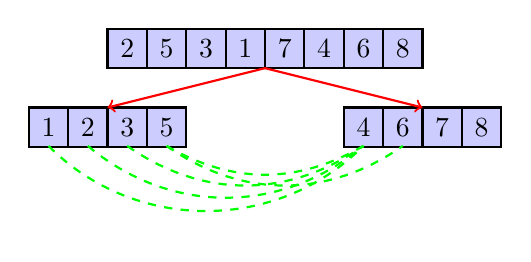
\begin{tikzpicture}[scale=1., auto,swap]
 
  \foreach \i/\name in { 0/2,1/5,2/3,3/1,4/7, 5/4, 6/6, 7/8 } {
         \draw[  fill=blue!20, thick ] (\i*0.5,0) rectangle (\i*0.5+0.5, 0.5);
         \node at (\i*0.5+0.25, 0.5/2) {$\name$};
 }

 %level 2
  
   \foreach \i/\name/\n in { 0/1/s1,1/2/s2,2/3/s3,3/5/s5} {
         \draw[  fill=blue!20, thick ] (\i*0.5-1,0-1) rectangle (\i*0.5-1+0.5, 0.5-1);
         \node (\n) at (\i*0.5+0.25-1, 0.5/2-1) {$\name$};
 }
 
    \foreach \i/\name/\n in { 4/4/s4, 5/6/s6, 6/7/s7, 7/8/s8} {
         \draw[  fill=blue!20, thick ] (\i*0.5+1,0-1) rectangle (\i*0.5+1+0.5, 0.5-1);
         \node (\n) at (\i*0.5+0.25+1, 0.5/2-1) {$\name$};
 }
 
  
 % lines 
 \foreach \source/\dest in {{( 4*0.5 , 0)/( 2*0.5 - 1, -0.5)}, {( 4*0.5 , 0)/( 6*0.5 + 1, -0.5)}} 
 	\path[draw=red, ->, thick]  \source  --  \dest;
 
\draw[green, dashed, thick] (s5.south) to [out=-30, in=180+30] (s4.south);
\draw[green, dashed, thick] (s3.south) to [out=-35, in=180+35] (s4.south);
\draw[green, dashed, thick] (s2.south) to [out=-40, in=180+40] (s4.south);
\draw[green, dashed, thick] (s1.south) to [out=-45, in=180+45] (s4.south);

\draw[green, dashed, thick] (s5.south) to [out=-35, in=180+35] (s6.south);


\end{tikzpicture}

\end{figure}

如图:1和4比较,$1<4$,那么1不需要在和4后面的数比较。

实际上我们只需要在归并排序的基础上就行修改就可得到逆序数的解决方法。其算法伪代码如下:

\begin{small} 

\noindent
{\sc Sort-and-Count}$(A)$
\begin{algorithmic}[1]
\STATE Divide $A$ into two sub-sequences $L$ and $R$;
\STATE $(RC_L, L)$ = {\sc Sort-and-Count}$(L)$;
\STATE $(RC_R, R)$ = {\sc Sort-and-Count}$(R)$;
\STATE $(C, A)$ = {\sc Merge-and-Count}$(L,R)$;
\RETURN{$ (RC=RC_L+RC_R+C, A);$}
\end{algorithmic}
{\sc Merge-and-Count} $(L,R)$
\begin{algorithmic}[1]
\STATE $RC = 0;$ $ i=0; $ $j=0;$
\FOR{ $k=0$ to $\|L\|+\|R\|-1$ }
	\IF { $L[i] > R[j] $}
		\STATE $A[k] = R[j];$
		\STATE $j++;$
		\STATE \textcolor{red}{$RC += (\frac{n}{2} - i);$}
	\ELSE 
		\STATE $A[k] = L[i];$
		\STATE $i++;$
	\ENDIF
\ENDFOR
\RETURN{ ($RC$, $A$); }
\end{algorithmic}
Time complexity: $T(n)=O(n\log n)$. 
\end{small} 

	在合并的函数中,比较左边的数L[i]和右边子数组的R[j],如果$L[i] > R[j]$,那么L[i]后面的数比R[j]都要大,因此逆序数个数增加了$ \frac{n}{2} -i$。

	逆序数问题的讨论:
	
	排序的过程实际上就是减少逆序数的过程,假设我们记录了排序过程中减少的逆序数的数量,那么就得到了所有的逆序数的数量。
	
\section{快速排序}
\subsection{快速排序的思想}
	快速排序和上次课讲的归并排序的思路比较像,但是分的办法不一样。

	快速排序的分法:随便选择一个元素$A[j]$,所有的其他元素和这个元素比较一次,那么就把比它小的放到 $S_{-}$,比它大的元素放到$S_{+}$。然后就是对$S_{-}$排序,对$S_{+}$排序。接着就输出$S_{-}$,$A[j]$,$S_{+}$。

	快速排序比归并排序的优势之一:代码比较简单。	虽然代码写起来容易,但是分析就比较难了。理想情况下,是一次分2半,但是因为选择的随机性,我们不知道将数组分成的比例是多少。
\begin{itemize}
 \item 
{\bf Worst-case:} 选择了最大或者最小的元素作枢纽元; 我们每次选择的都是数组中最大或者最小的数,分类操作需要一次循环,因此合并操作需要$O(n)$的时间。那么复杂度就是$O(n^2)$。


\begin{center}
$T(n) \leq T(n-1) + cn \Rightarrow T(n) = O(n^2)$
\end{center}

\ \\
\item 
{\bf Best-case:} 选择了中间元素作枢纽元;那么复杂度是$O(n \log n)$。

\begin{center}
$T(n) \leq 2T(n/2) + cn \Rightarrow T(n) = O(n \log n)$
\end{center}

\ \\
\item 
{\bf Most cases:} 事实上,我们选择的情况不是最好也不是最差,只会是一般的情况。我们接下来证明期望值是$T(n) = O(n \log n)$。

%$T(n) \leq T(n/4) + T(3/4 n) + cn \Rightarrow T(n) = O(n \log n)$. \\
\end{itemize}
\subsection{快速排序复杂度$O(n \log n)$的证明}
	我们在计数过程中只关心两两比较的次数,用X表示对大小为N的数组排序比较的次数。

\begin{enumerate}
\item
第一个观察:任意i和j 最多比较一次,假如选择了元素4,4和所有元素比了一次,那么4以外的元素都被划分到了2个子数组,4不会再和其他元素比较。下面计算快速排序算法比较次数的期望值。
\begin{figure}[H]
\centering
    
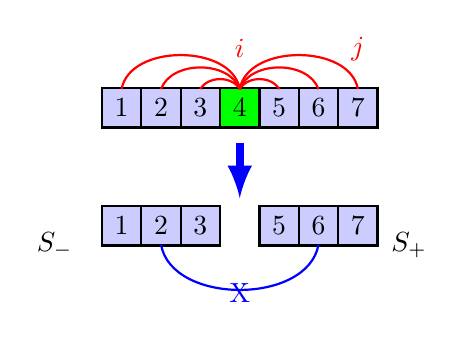
\begin{tikzpicture}[scale=1., auto,swap]
 
  \foreach \i/\name in { 0/1,1/2,2/3,3/4,4/5, 5/6, 6/7} {
         \draw[  fill=blue!20, thick ]  (\i*0.5,0) rectangle (\i*0.5+0.5, 0.5);
         \node (U\name) at (\i*0.5+0.25, 0.5/2 ) {$\name$};
 }

 
   \foreach \i/\name in { 3/4} {
         \draw[  fill=green, thick ]  (\i*0.5,0) rectangle (\i*0.5+0.5, 0.5);
         \node (U\name) at (\i*0.5+0.25, 0.5/2 ) {$\name$};
 }
 
 %level 2
  
   \foreach \i/\name in { 0/1,1/2,2/3 } {
         \draw[  fill=blue!20, thick ]  (\i*0.5 ,0-1.5) rectangle (\i*0.5 +0.5, 0.5-1.5);
         \node (B\name) at (\i*0.5+0.25 , 0.5/2-1.5) {$\name$};
 }
 
    \foreach \i/\name in { 4/5, 5/6, 6/7 } {
         \draw[  fill=blue!20, thick ]   (\i*0.5  ,0-1.5) rectangle (\i*0.5 +0.5, 0.5-1.5);
         \node (B\name) at (\i*0.5+0.25 , 0.5/2-1.5) {$\name$};
 }
 %arrow
 \draw[blue, -latex, line width=3pt] (4*0.5-0.25, -0.2) -- (4*0.5-0.25, -0.9);
  %arc
  \draw[red, thick] (U4.north) to [out=60,in=180-60] (U5.north);
  \draw[red, thick] (U4.north) to [out=70,in=180-70] (U6.north);
  \draw[red, thick] (U4.north) to [out=80,in=180-80] (U7.north);	
  
    \draw[red, thick] (U4.north) to [out=180-60,in=60] (U3.north);
  \draw[red, thick] (U4.north) to [out=180-70,in=70] (U2.north);
  \draw[red, thick] (U4.north) to [out=180-80,in=80] (U1.north);	
  
    \draw[blue, thick] (B2.south) to [out=-80,in=260] (B6.south);	
    
   %no comparison 
   \node[blue, thick] at (4*0.5-0.25, -2.1) {X};
    \node[red, thick] at (4*0.5-0.25, 1) {$i$};
      \node[red, thick] at (7*0.5-0.25, 1) {$j$};
     \node[ thick] at (-0.6, -1.5) {$S_{-}$};
         \node[ thick] at (7*0.5 + 0.4, -1.5) {$S_{+}$};
\end{tikzpicture}

\end{figure}

\begin{itemize}

      \item 定义 $X_{ij} = I \{ A[i] \text{ is compared with } A[j] \}$.如果$A[i]$ 和$A[j]$比较了,$X_{ij}=1$,否则$X_{ij}=0$。
      \item 因此 $X = \sum_{i=0}^{n-1}\sum_{j=i+1}^{n-1} X_{ij}$. 
      \begin{eqnarray}
      E[ X ] & = &  E [\sum_{i=0}^{n-1}\sum_{j=i+1}^{n-1} X_{ij} ] \nonumber \\
              & = &   \sum_{i=0}^{n-1}\sum_{j=i+1}^{n-1} E[ X_{ij} ] \nonumber \\
              & = &   \sum_{i=0}^{n-1}\sum_{j=i+1}^{n-1} Pr\{ A[i]  \text{ is compared with } A[j]\}  \nonumber 
      \end{eqnarray} 

\end{itemize} 

\item
	第二个观察:当我们在处理$A[i, i+1, ... , j]$数组的时候,A[i] 和 A[j]比较发生的条件是:$A[i]$或者 $A[j]$其中一个元素被选择作为枢纽元(划分数组的元素)。如果都没有被选中过,那么不会被比较。

	例如:对于1,2,3,4,5这个数组,1和5比较的条件是1或者5被选择,假如选择2,3,4,那么1和5会被分到2个不同的子数组,就不会被比较。而且1和5比较的概率此时是2/5。当i,j不是数组的边界时,这个概率小于$\frac{2}{j-i+1}$,因此$Pr\{A[i]  \text{ is compared with } A[j]\}  \leq \frac{2}{j-i+1}$。

\end{enumerate}

	那么我们重新计算前面的比较次数期望。
 	\begin{eqnarray}
      E[ X ]        & = &   \sum\nolimits_{i=1}^{n}\sum\nolimits_{j=i+1}^n Pr\{ A[i]  \text{ is compared with } A[j]\}  \nonumber \\
      & \leq &  \sum\nolimits_{i=1}^{n}\sum\nolimits_{j=i+1}^n  \frac{2}{j-i+1} \nonumber \\ 
      & = & \sum\nolimits_{i=1}^n \sum\nolimits_{k=1}^{n-i} \frac{2}{k+1}  \nonumber \\        
      & < & \sum\nolimits_{i=1}^n \sum\nolimits_{k=1}^{n} \frac{2}{k+1} \nonumber \\
      & = & O( n \log n ) \nonumber 
      \end{eqnarray} 
\subsection{改造快速排序}
	我们把算法改造一下,让我们的分析更加简单。
	
\begin{small}
\centering
{\sc ModifiedQuickSort}$(A)$
\begin{algorithmic}[1]
\WHILE{ TRUE }
\STATE \textcolor{red}{randomly} choose a splitter $A[j]$;
\FOR { $i=0 $ to $n-1$ }
\STATE Put $A[i]$ in $S_{-}$ if $A[i] <  A[j]$;
\STATE Put $A[i]$ in $S_{+}$ if $A[i] > A[j]$;
\ENDFOR
\IF { $\|S_{+}\| > \frac{n}{4} $ and $\|S_{-}\| > \frac{n}{4}$ }
\STATE break;
\ENDIF
\ENDWHILE
\STATE {\sc ModifiedQuickSort}$(S_{+})$;
\STATE {\sc ModifiedQuickSort}$(S_{-})$;
\STATE Output $S_{-}$, then $A[j]$, and finally $S_{+}$; 
\end{algorithmic}
\end{small}

	我们在前面加了一个死循环,随机选择一个元素,并将整个数组分成2部分:$S_{-}$和$S_{+}$。如果2个子数组的大小都比n/4要大,那么我们决定选择这个元素作枢纽;否则我们重新选择一个元素直到满足条件。


\begin{figure}[H]
\centering
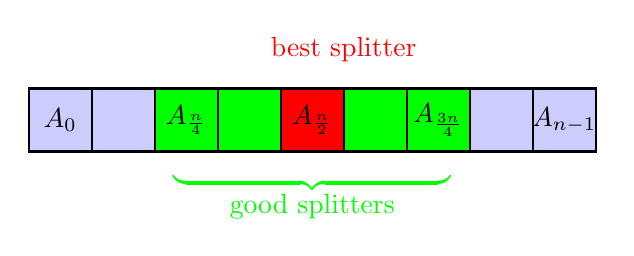
\begin{tikzpicture}[scale=1., auto,swap]
 
  \foreach \i/\name in { 0/A_0,1/\hdots,2/A_{\frac{n}{4}},3/\hdots,4/A_{\frac{n}{2}},5/\hdots,6/A_{\frac{3n}{4}},7/\hdots,8/A_{n-1}}{
           \draw[  fill=blue!20, thick ] (\i*0.8,0) rectangle (\i*0.8+0.8, 0.8);
         \node at (\i*0.8+0.4, 0.8/2) {$\name$};
 }

  \foreach \i/\name in { 2/A_{\frac{n}{4}},3/\hdots,4/A_{\frac{n}{2}},5/\hdots,6/A_{\frac{3n}{4}}}{
           \draw[  fill=green, thick ] (\i*0.8,0) rectangle (\i*0.8+0.8, 0.8);
         \node at (\i*0.8+0.4, 0.8/2) {$\name$};
 }
 
   \foreach \i/\name in {4/A_{\frac{n}{2}}}{
           \draw[  fill=red, thick ] (\i*0.8,0) rectangle (\i*0.8+0.8, 0.8);
         \node at (\i*0.8+0.4, 0.8/2) {$\name$};
 }
 \node[red] at (5*0.8, 1.3) {best splitter};
 \node[green] at (5*0.8-0.4, -0.4) {$\underbrace{\qquad\qquad\qquad\qquad\qquad}$};
 \node[green] at (5*0.8-0.4, -0.7) {good splitters};
 
 
\end{tikzpicture}
\end{figure}

\begin{enumerate}
\item 选中中间元素$A[n/2]$ 的概率是$ \frac{1}{n}$
\item 选中中间部分(绿色部分)的概率是$ \frac{1}{2}$。2项分布的概率是$ \frac{1}{2}$,那么期望是2.也就是循环2次就可以找到中间部分的枢纽元。那么合并的时间就是2n。$T(n) = T(n/4)+T(3n/4)+2n$的复杂度是$O(n\log n)$。
\item 总结: 
	\begin{itemize} 
 \item 迭代深度是$O( \log_{ \frac{4}{3}} n )$.
 \item 每一次迭代找枢纽元的时间是$O(n)$. 
%\item Notation: a subproblem has a ``type'' of $j$ if its size is $j$. 
%\item How many types of subproblems? $\log _{\frac{4}{3}} n$  
%\item How many subproblems in each type? $(\frac{4}{3})^{j+1}$ subproblems in type $j$. 
%\item Running time of each subproblem: $O( n (\frac{3}{4})^{j+1} )$;
\item  $T(n) = O(n \log_{\frac{4}{3}} n )$.
	\end{itemize}
\end{enumerate}

\section{乘法问题}
一般做法如下图所示:
\begin{figure}[H]
\centering
 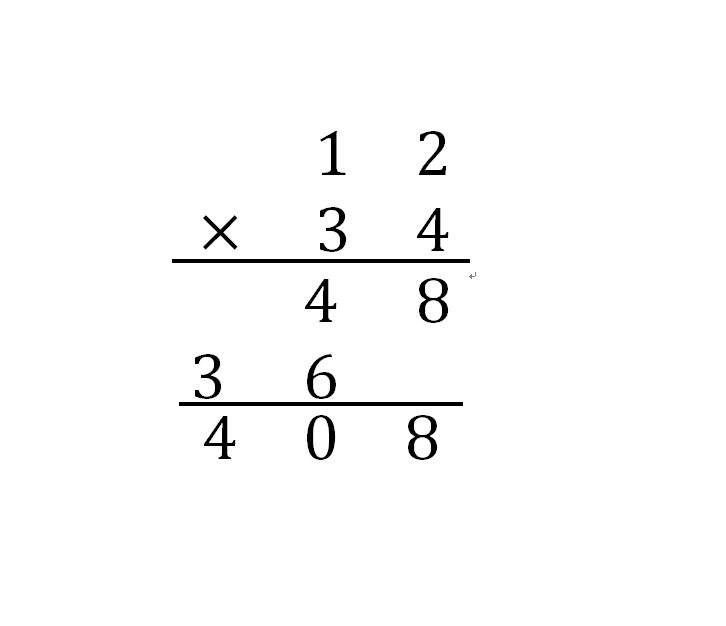
\includegraphics[width=2.5in,height=1.5in] {multiply.png}
		
\end{figure}
提出问题:$O(n^2)$的复杂度是最优的吗?


\subsection{解决方法1}

\begin{itemize}
\item 
	重要观察:2个整数x,y可以表示成n位的二进制数,可以分成2部分。
\item 
	分治策略: 
\begin{enumerate}
 \item {\bf Divide:} $x=x_h \times 2^{\frac{n}{2}} + x_l$, $y=y_h \times 2^{\frac{n}{2}} + y_l$, 
 \item {\bf Conquer:} calculate $x_h y_h$, $x_h y_l$, $x_l y_h$, and $x_l y_l$;  
 \item {\bf Combine:} 
\begin{eqnarray}
                 xy &=& (x_h \times 2^{\frac{n}{2}} + x_l) (y_h \times 2^{\frac{n}{2}} + y_l) \\
                    &=& x_hy_h 2^n + ( x_hy_l + x_ly_h) 2^{\frac{n}{2}} + x_l y_l 
                \end{eqnarray} \\
\end{enumerate}
\end{itemize}

	举例分析:计算 12 × 34
\begin{itemize}
	\item	Objective: to calculate $12 \times 34 $
	\item $x=12 = 1 \times 10 + 2$, $y= 34 =3\times 10 + 4$
	\item $x\times y = (1 \times 3)\times 10^2 + ( (1 \times 4)+(2\times 3))\times 10 + 2\times 4 $
\end{itemize}
	这个算法的复杂度:我们将其分成4个子问题,每个子问题的规模是$ \frac{n}{2}$,3次加法。$T(n)=4T(n/2) + cn \Rightarrow T(n)=O(n^2)$。如下表所示。
	
\begin{table}[H]
\centering
   \begin{tabular}{|c||c|c|}\hline
   \hline
             $\times$  &  $y_{h}$ & $y_{l}$  \\
  \hline \hline
  	$x_{h}$ & $x_{h} y_{h}$ & $x_{h}y_{l}$ \\
  \hline
  	$x_{l}$ & $x_{l} y_{h}$ & $x_{l}y_{l}$ \\
  \hline
  \end{tabular}
\end{table}

	我们可以发现以下问题:
 \begin{itemize}
 	\item 我们的目标是计算 $x_hy_h 2^n + ( x_hy_l + x_ly_h) 2^{\frac{n}{2}} + x_l y_l $。
	\item 我们发现没必要分别计算  $x_hy_l$ 和  $x_ly_h$,只需要计算 $( x_hy_l + x_ly_h)$。
	\item 很明显 $( x_hy_l + x_ly_h) + ( x_hy_h + x_ly_l) = (x_{h}+x_{l}) \times (y_{h} + y_{l}) $。 
	所以$( x_hy_l + x_ly_h)$ 只需要一次额外的乘法就能计算出来。 
 \end{itemize} 	 

\subsection{新的分治算法}

\begin{itemize}
 \item \textcolor{blue}{\bf Divide:} $x=x_h \times 2^{\frac{n}{2}} + x_l$, $y=y_h \times 2^{\frac{n}{2}} + y_l$, 
 \item \textcolor{blue}{\bf Conquer:} 计算 $x_h y_h$, $x_l y_l$, 和 $P=(x_h + x_l) (y_h + y_l)$;  
 \item \textcolor{blue}{\bf Combine:} \begin{eqnarray}
                 xy &=& (x_h \times 2^{\frac{n}{2}} + x_l) (y_h \times 2^{\frac{n}{2}} + y_l) \\
                    &=& x_hy_h 2^n + ( x_hy_l + x_ly_h) 2^{\frac{n}{2}} + x_l y_l \\
		    &=& x_hy_h 2^n + ( P - x_hy_h - x_l y_l) 2^{\frac{n}{2}} + x_l y_l 
                \end{eqnarray} \\
\end{itemize}


	还是刚才那个例子:计算12 × 34
\begin{enumerate}
	\item	Objective: to calculate $12 \times 34 $
	\item $x=12 = 1 \times 10 + 2$, $y=34=3 \times 10 +4$
	\item $P=(1 + 2)\times(3 + 4)$ 
	\item $x\times y = (1\times 3)\times 10⋯⋯2 + ( P - 1\times3 - 2 \times 4)  \times 10 + 2\times 4 $
\end{enumerate}
	这个算法可以分成3个子问题,6次加法,2次移位。
那么算法的复杂度变成$T(n)=3T(n/2) + cn \Rightarrow T(n)=O(n^{\log_2 3}) = O(n^{1.585})$。

\subsection{算法性能的比较}
	那么这个算法到底怎么样呢?
	
	对于n很大时,Karatsuba的算法效果是很明显的。但是当n的规模比较小时,额外的移位和加法操作将使这个算法变慢。	当使用快速傅立叶变换的技术,乘法时间复杂度是$O(n\log n)$ 。 
\begin{figure}[H]
\centering
 		\includegraphics[width=2.5in,height=1.5in] {L5-karatsuba-experiment.eps}
\end{figure}

\subsection{扩展:快速除法}

\begin{enumerate}
\item
	问题: 给定2个n位的数 s 和 t, 计算$ q=s/t$ 和$r=s mod t$。
\item
	方法: 
	\begin{itemize}
	\item 先用牛顿法 $x_{i+1} =  2 x_i - t \times x_i^2 $ 计算 $ x = 1 / t$ 。

	\item 最多需要 $\log n$ 次迭代。

	\item	除法和乘法速度一样快。 
	\end{itemize}
\item
	牛顿迭代法的细节
	\begin{itemize}
	 \item  $f(x) = (t - \frac{1}{x})$,$x$ 是 $f(x) = 0$ 的解。
	  \item 牛顿迭代法: 
 	\begin{eqnarray}
		 x_{i+1} &=& x_i - \frac{f(x_i)}{f'(x_i)} \\
         &=& x_i - \frac{t-\frac{1}{x_i}}{ \frac{1}{x_i^2} } \\
         &=& - t\times x_i^2 + 2 x_i 
 	\end{eqnarray}
	 \item 牛顿迭代法的迭代速度:迭代次数只需要 $\log \log t = O(\log n)$。
\end{itemize}
\item 
	举例分析:计算$ \frac{1}{13}$
\begin{center} 
\begin{tabular}{ l r r } 
\hline \\
\#Iteration & $x_i$ & $\epsilon_i$ \\ 
\hline 
 0	&0.018700	&-0.058223 \\
1	&0.032854	&-0.044069  \\
2	&0.051676	&-0.025247 \\
3	&0.068636	&-0.008286 \\
4	&0.076030	&-0.000892 \\
5	&0.076912	&-1.03583e-05 \\
6	&0.076923	&-1.39483e-09 \\
7	&0.076923	&-2.77556e-17 \\
8	&...	&... \\
 \hline
\end{tabular}
\end{center} 
	
\end{enumerate}
	
	
\section{矩阵乘法}
问题: 给定2个 $n \times n $矩阵 $A$ 和$ B$, 计算 $C = AB$。 
\subsection{解决方法1}
	
	一般的方法: $A$的第$i$行 和$ B$的第$j$列相乘得到$C_{ij}$,复杂度是$O(n^3)$。因为根据定义矩阵C中每个元素都需要$O(n)$次乘法,总共有$n$个元素。
	
	关键观察:将矩阵分成4块,每一块是 $\frac{n}{2} \times \frac{n}{2}$ 的大小。
	
	分治算法:
\begin{enumerate}
 \item {\bf Divide:}  把 $A$, $B$, 和 $C$分别划分成4个小矩阵 ; 
 \item {\bf Conquer:}  计算子矩阵的乘积; 
 \item{\bf Combine:} 
\[ 
\begin{matrix}
\begin{pmatrix}
C_{11} & C_{12} \\ 
C_{21} & C_{22} 
\end{pmatrix}
=
\begin{pmatrix}
A_{11} & A_{12} \\ 
A_{21} & A_{22}  
\end{pmatrix}

\begin{pmatrix}
B_{11} & B_{12} \\ 
B_{21} & B_{22}  
 
\end{pmatrix}
    
   \end{matrix}
\]


\begin{eqnarray}
 C_{11} &=& (A_{11}\times B_{11}) + (A_{12} \times B_{21}) \\
C_{12} &=& (A_{11}\times B_{12}) + (A_{12} \times B_{22}) \\
C_{21} &=& (A_{21}\times B_{11}) + (A_{22} \times B_{21}) \\
C_{22} &=& (A_{21}\times B_{12}) + (A_{22} \times B_{22}) 
\end{eqnarray}

 
\end{enumerate}

	算法的复杂度:每个问题分成8个子问题和4次加法。每次加法花费$O(n^2)$时间。
所以时间复杂度是:$T(n)=8T(n/2) + cn^2 \Rightarrow T(n)=O(n^3)$
	
	问题:能降低矩阵乘法的复杂度吗?
\subsection{Strassen 算法}
	Strassen 算法:第一次提出的算法比O(n3)要快。
	
\subsubsection{算法的主要思想}
	减少求解子问题的数目:8个子问题的结果并不一定都需要,只需要算出7个矩阵的结果就能表示出来。
\[ 
\begin{matrix}
\begin{pmatrix}
C_{11} & C_{12} \\ 
C_{21} & C_{22} 
\end{pmatrix}
=
\begin{pmatrix}
A_{11} & A_{12} \\ 
A_{21} & A_{22}  
\end{pmatrix}

\begin{pmatrix}
B_{11} & B_{12} \\ 
B_{21} & B_{22}  
 
\end{pmatrix}
    
\end{matrix}
\]

\begin{eqnarray}
P_1 = A_{11} \times (B_{12} - B_{22} ) \\
P_2 = ( A_{11} + A_{12} ) \times B_{22} \\
P_3 = ( A_{21} + A_{22} ) \times B_{11} \\
P_4 = A_{22} \times (B_{21} - B_{11} ) \\
P_5 = ( A_{11} + A_{22} ) \times (B_{11} + B_{22} ) \\
P_6 = (A_{12} - A_{22} )\times (B_{21} + B_{22} ) \\
P_7 = (A_{11} - A_{21} ) \times (B_{11} + B_{12} ) 
\end{eqnarray}



\begin{eqnarray}
C_{11} &=& P_4 + P_5 + P_6 - P_2  \\
C_{12} &=& P_1 + P_2\\
C_{21} &=& P_3 + P_4 \\
C_{22} &=& P_1 + P_5 - P_3 - P_7 
\end{eqnarray}

\subsubsection{Strassen算法的复杂度}
	那么Strassen算法的复杂度是$T(n)=7T(n/2) + cn^2 \Rightarrow T(n)=O(n^{\log_2 7}) = O(n^{2.807})$。

\subsubsection{Strassen算法的优劣}	
\begin{itemize}
\item {\bf 优势:}\\
	1.比一般的算法速度快很多。

	2.Strassen算法可以用来解决其他问题:矩阵求逆,行列式求值,图的三角形个数计数。
\item {\bf 劣势:}\\
	1.只对于规模较大的问题复杂度有所提升。
	
	2.稳定性不足。
	
	3.相对于其他算法要求更多的内存资源。
\end{itemize}

\subsection{快速矩阵算法的进展}
\begin{itemize}
 \item multiply two $2 \times 2$ matrices: 7 scalar sub-problems: $O(n^{\log_2 7}) = O(n^{2.807})$ [ Strassen 1969 ]
 \item multiply two $2 \times 2$ matrices: 6 scalar sub-problems: $O(n^{\log_2 6})=O(n^{2.585})$ \textcolor{red}{(impossible)}[Hopcroft and Kerr 1971] 
\item multiply two $3 \times 3$ matrices: 21 scalar sub-problems: $O(n^{\log_3 21})=O(n^{2.771})$ \textcolor{red}{(impossible)}
\item multiply two $20 \times 20$ matrices: 4460 scalar sub-problems: $O(n^{\log_{20} 4460})=O(n^{2.805} )$ 
\item multiply two $48 \times 48$ matrices: 47217 scalar sub-problems: $O(n^{\log_{48} 47217 })=O(n^{2.780})$ 
\item Best known: $O(n^{2.376})$ [Coppersmit-Winograd, 1987]
\item Conjecture: $O( n^{2+\epsilon} )$ for any $\epsilon > 0$; 
\end{itemize}

\section{最近点对问题}
\begin{itemize}
\item
 {\bf INPUT: } 平面上的$n$个点  
\item
 {\bf OUTPUT: } 欧式距离最近的点对。
\end{itemize}

\begin{figure}[H]
\centering
 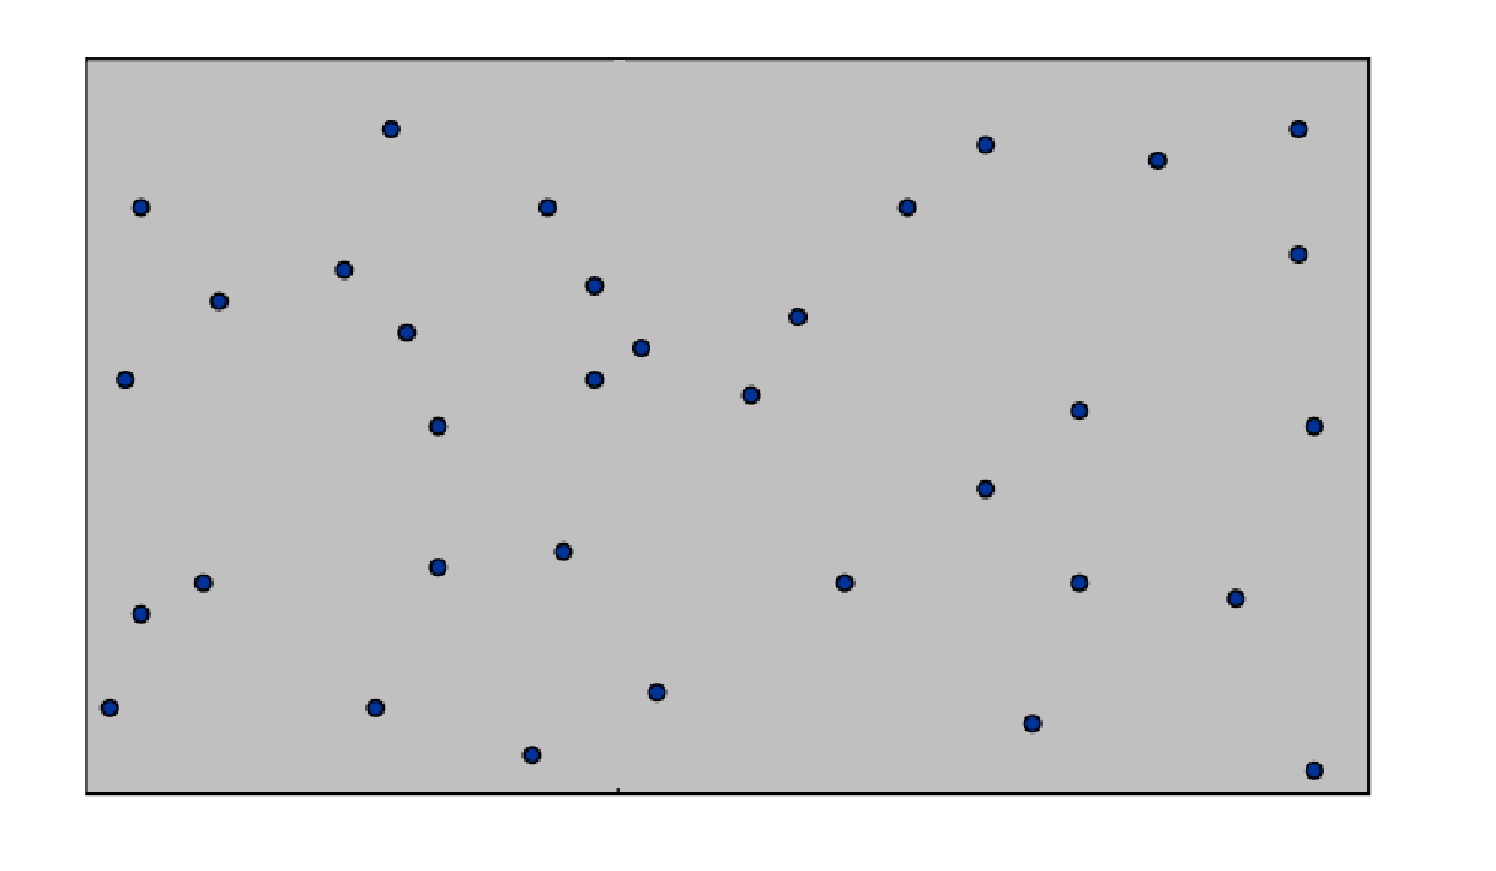
\includegraphics[width=3in] {L5-closestpair-example.eps}
\end{figure}
\begin{itemize}
 \item 
	直线上:将点进行排序,找出2个距离最近的点,复杂度是O(n log n) 。
\item
	平面上:比较所有的点对,需要O(n2) 的时间。
\end{itemize}
	问题:能够找出更快的算法吗?
\subsection{解决方案}
\subsubsection{方案1:分成4个子问题}
\begin{figure}[H]
\centering
 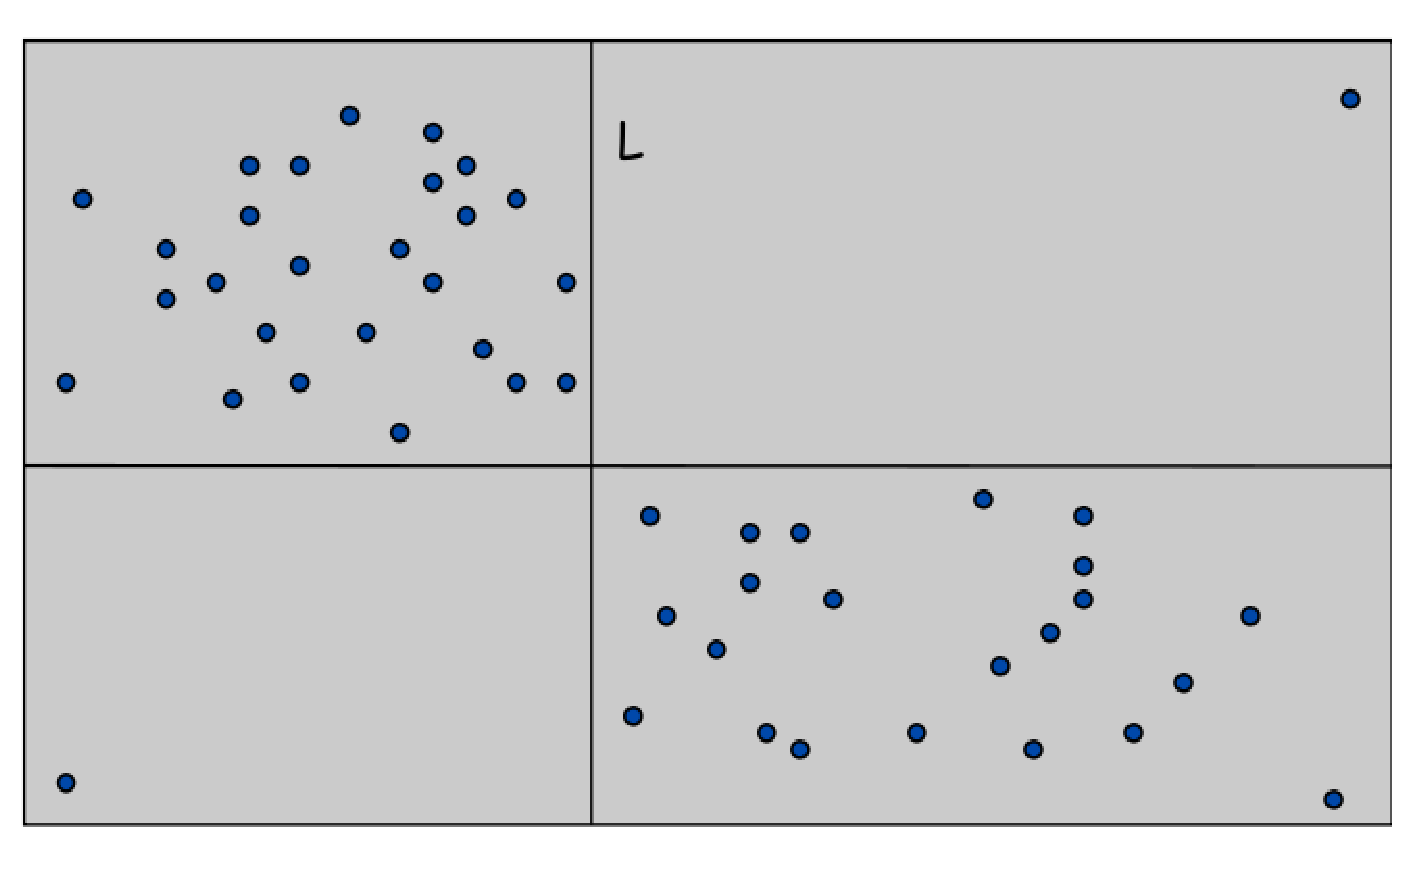
\includegraphics[width=3in] {L5-closestpair-4subsets.eps}
\end{figure}
	
	困难:分成的子集可能是不均衡的。我们无法保证每个子集都有差不多$ n/4 $个点。因此可能需要$O(n^2)$ 的时间去合并子集,最后的算法迭代表达式可能是这样的: $T(n) = 2 T(\frac{n}{2}) + O(n^{2})$ 。
	
\subsubsection{方案2:分成2个子问题}
	
	解决方法:很容易将所有的点安装x坐标进行排序,然后用$x_{ \lfloor \frac{n}{2} \rfloor }$ 将所有点分成2半。
\begin{itemize}
\item  {\bf Divide: }将所有点分成2半; 
\item  {\bf Conquer: }找出每个子问题的解:左半部分的最近点对,右半部分的最近点对; 
\item  {\bf Combine: }最近点对可能存在于边界左边一点和右边一点的情况。

\begin{figure}[H]
\centering
 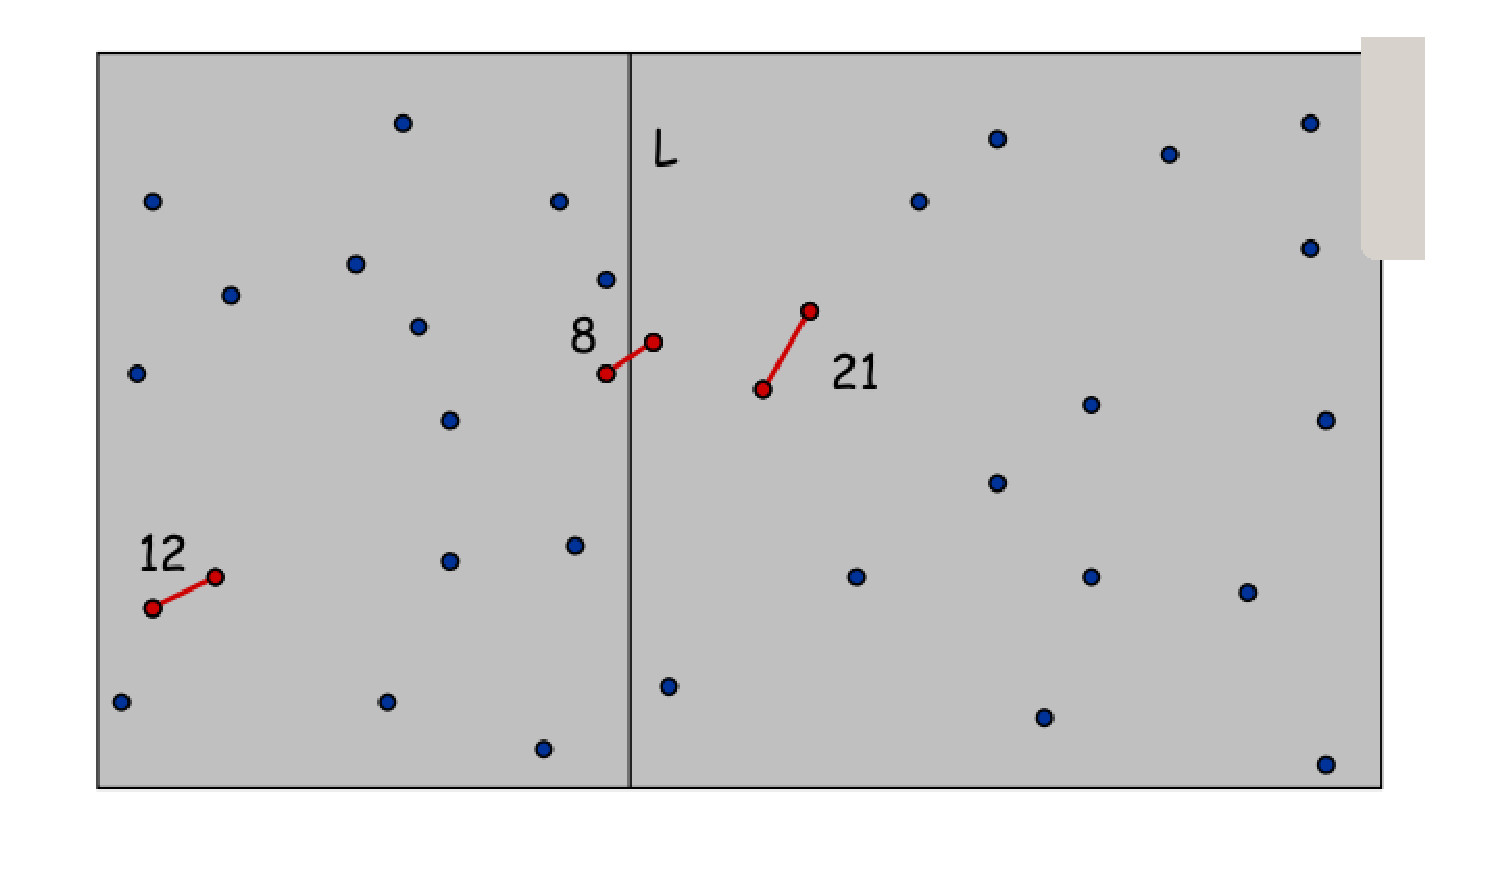
\includegraphics[width=3in] {L5-closestpair-12218.eps}
\end{figure}
	如果对左半边的每个点和右半边的每个点都做计算,那么时间开销很大:需要$O(n^2)$的时间。
\end{itemize}

	观察1:实际上,我们只需要观察L条带里面的点对的距离。那么条带的范围是$2\delta$,$\delta$ 
是取左边的最近点对和右边的最近点对的距离的较小者。如图所示,$\delta = \min(12,21)$。
\begin{figure}[H]
\centering
 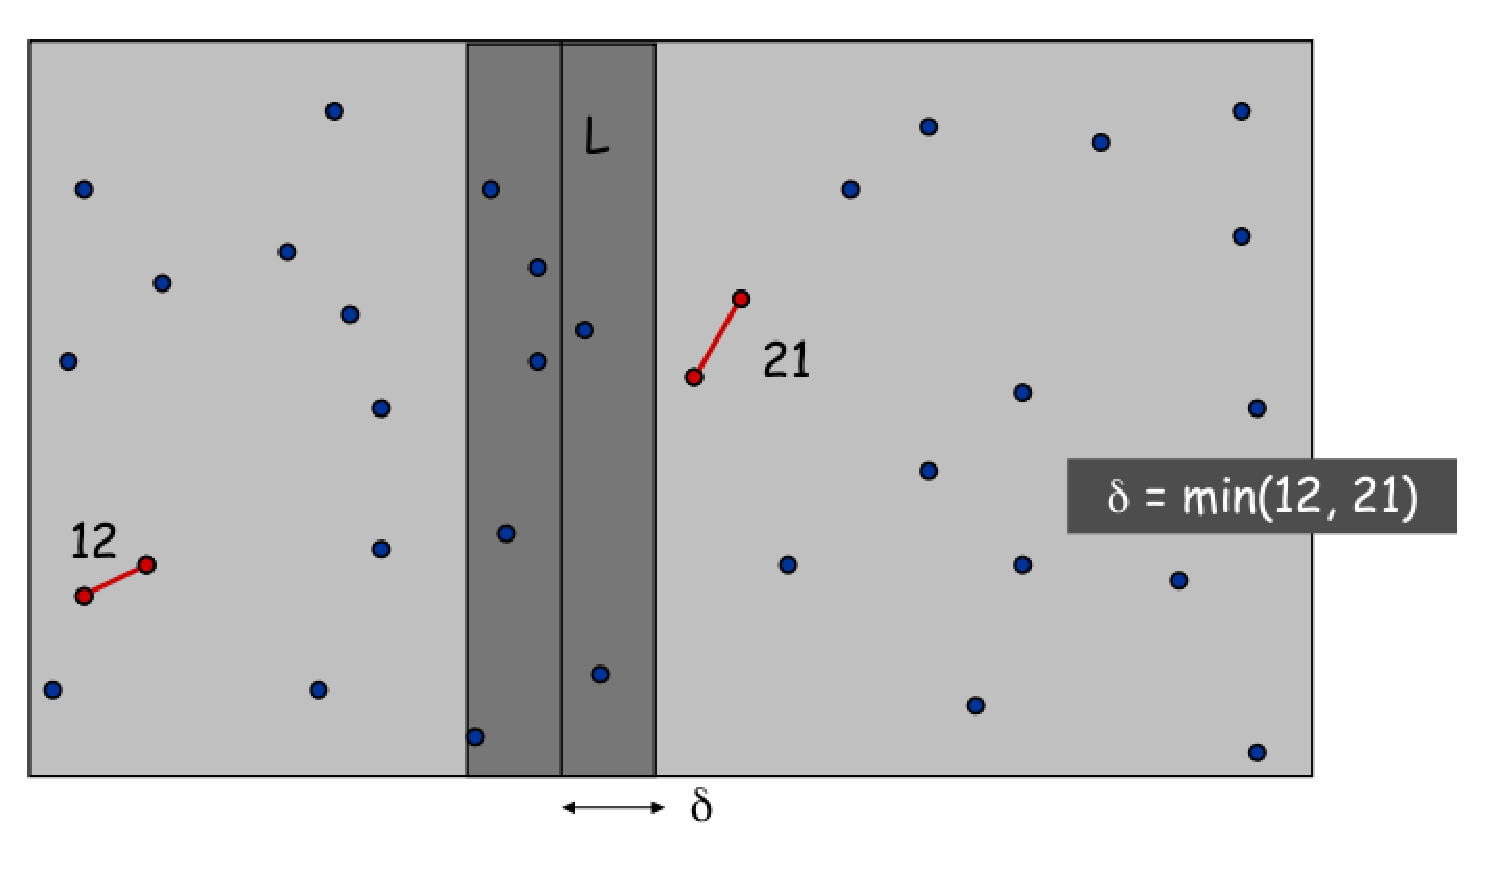
\includegraphics[width=3in] {L5-closestpair-1221delta-strip.eps}
\end{figure}

	观察2:即使在条带里面也没必要两两之间去计算。对中间的条带进行分割,每个格子的边长是$\delta/2$。	显然,一个格子里面只能装一个点。原因:当2个点在一个格子里面时,它们的距离将会小于$\delta$。
\begin{figure}[H]
\centering
 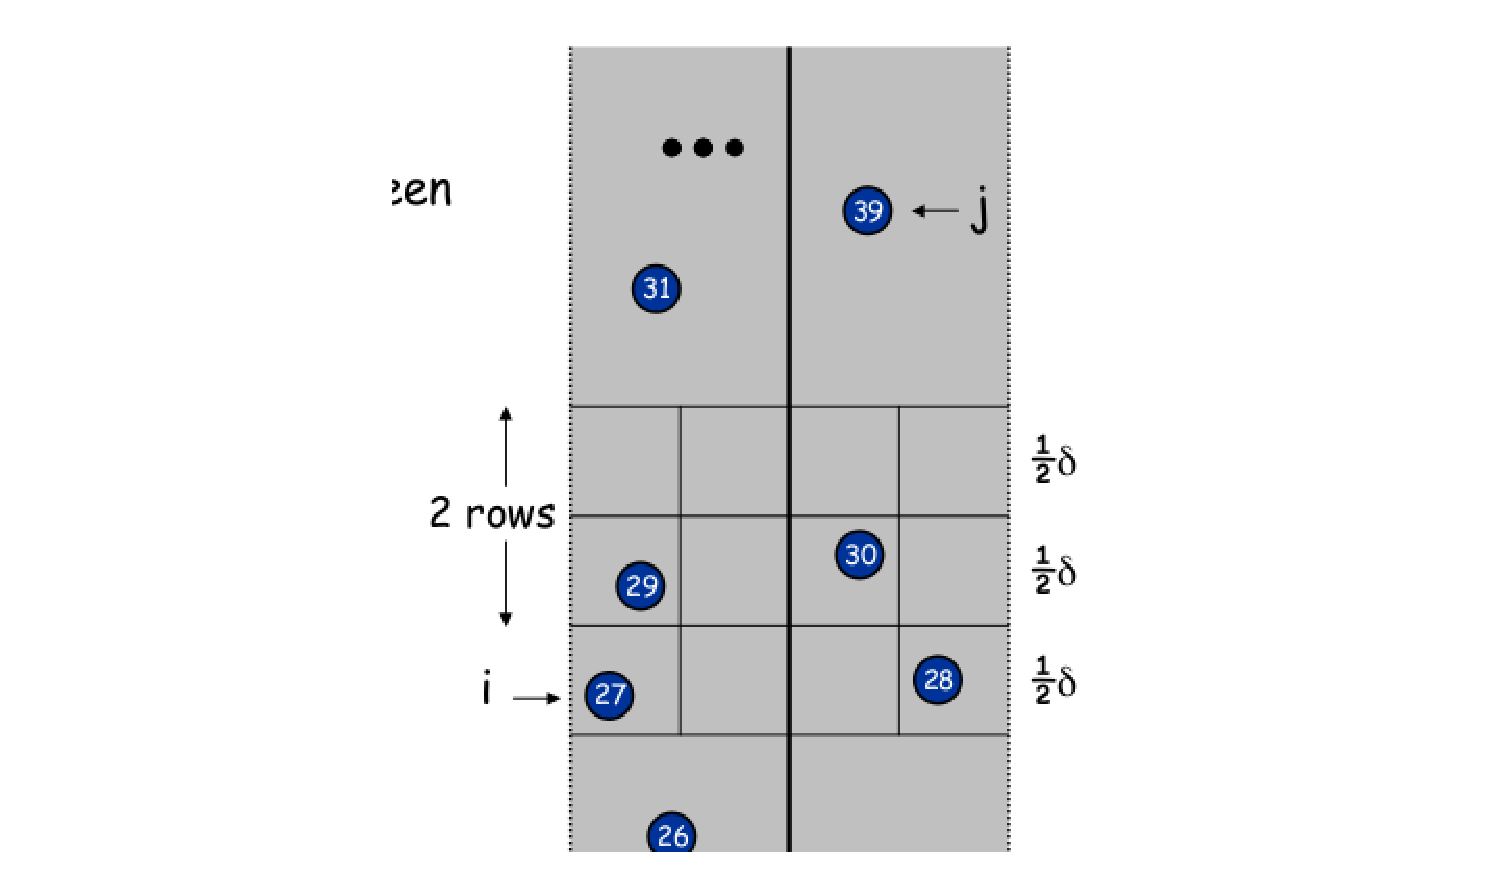
\includegraphics[width=2.6in] {L5-closestpair-1221delta-strip-7-reason.eps}
\end{figure}
	接下来分析可能出现的最近点对的计算,下面4种情况是可能出现的最近点对的情况。每幅图中绿色的点只需要和红色的点继续比较即可。
	
\begin{figure}[H]
\centering
 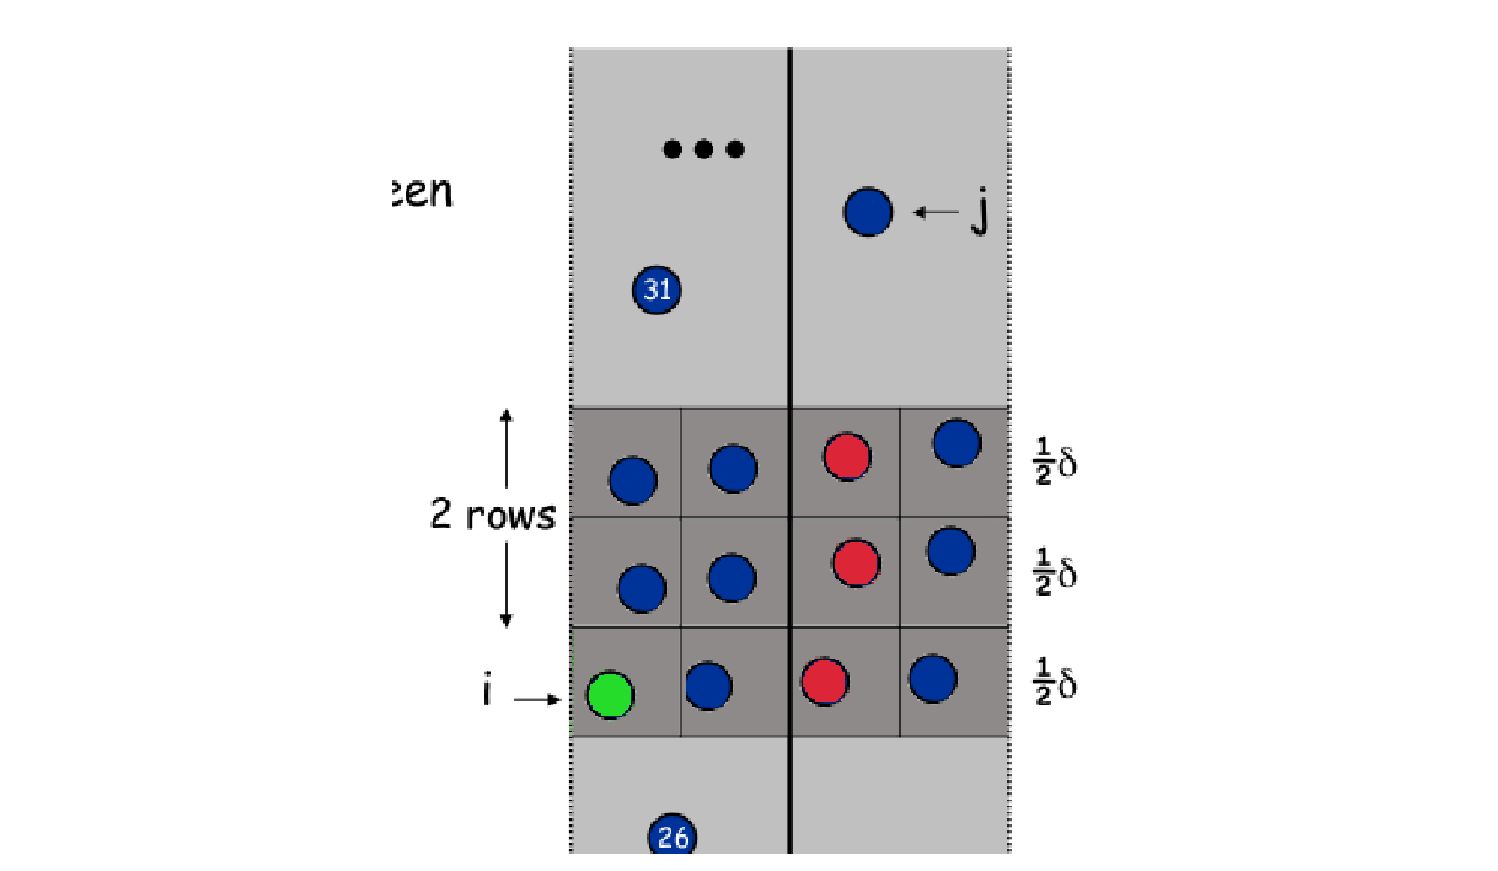
\includegraphics[width=3in] {L5-closestpair-1221delta-strip-7-reason1.eps}
\end{figure}

\begin{figure}
\centering
 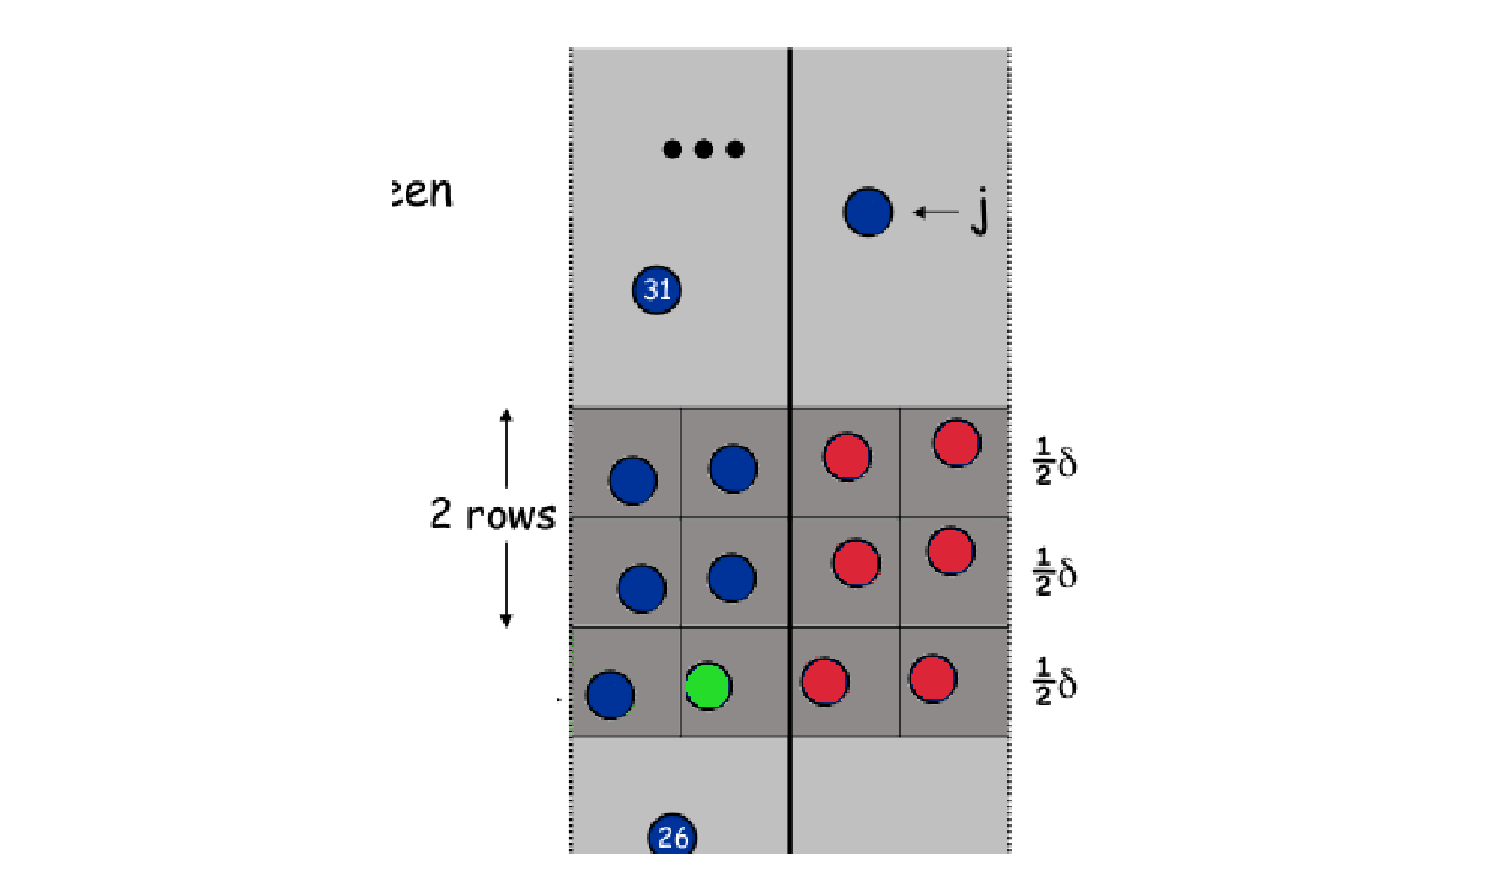
\includegraphics[width=3in] {L5-closestpair-1221delta-strip-7-reason2.eps}
\end{figure}

\begin{figure}[H]
\centering
 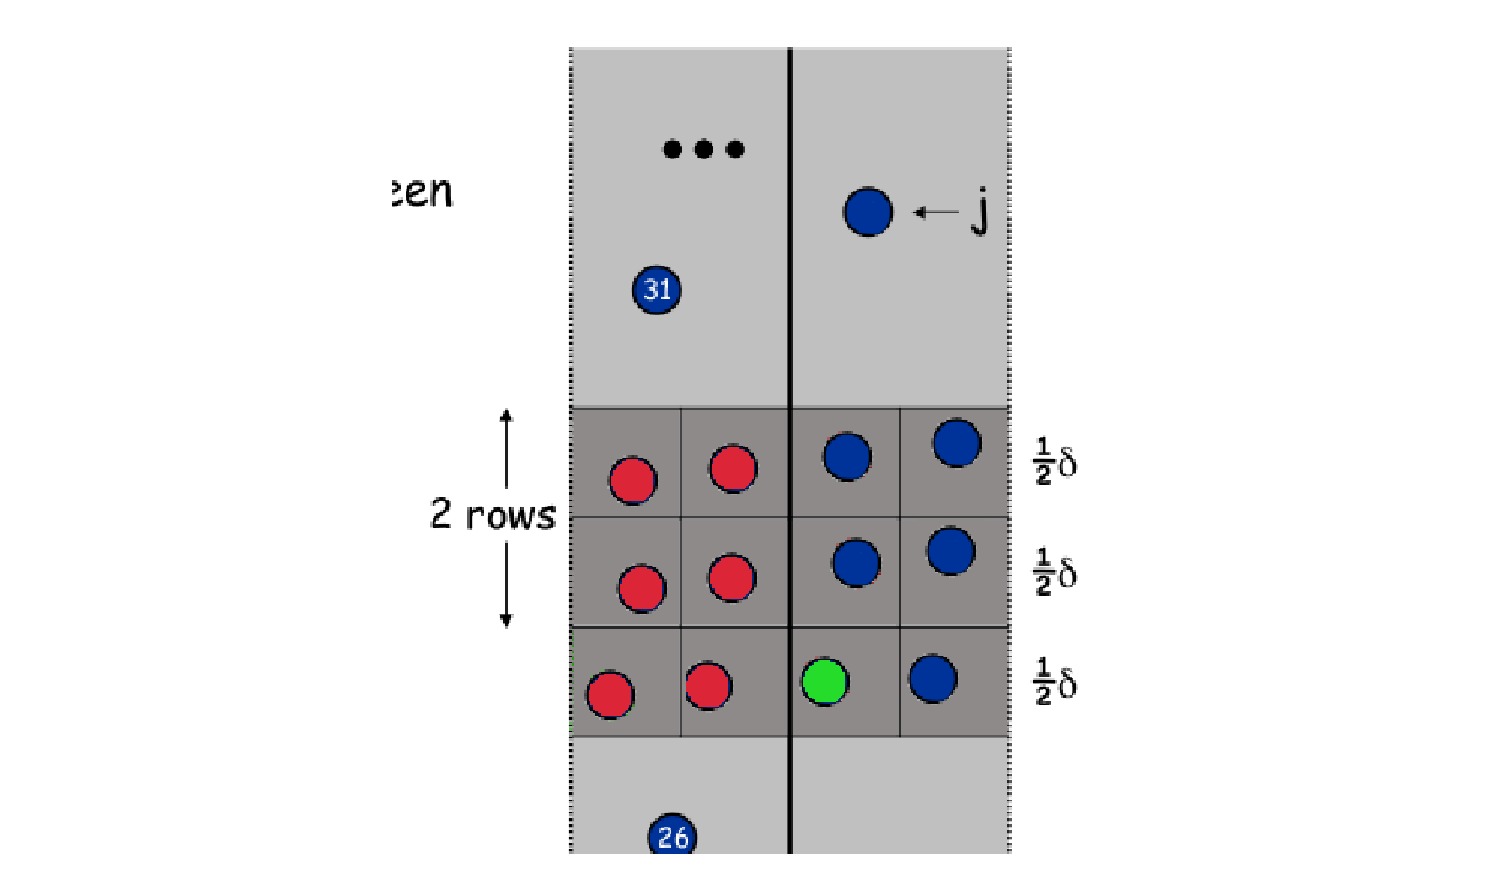
\includegraphics[width=3in] {L5-closestpair-1221delta-strip-7-reason3.eps}
\end{figure}

\begin{figure}[H]
\centering
 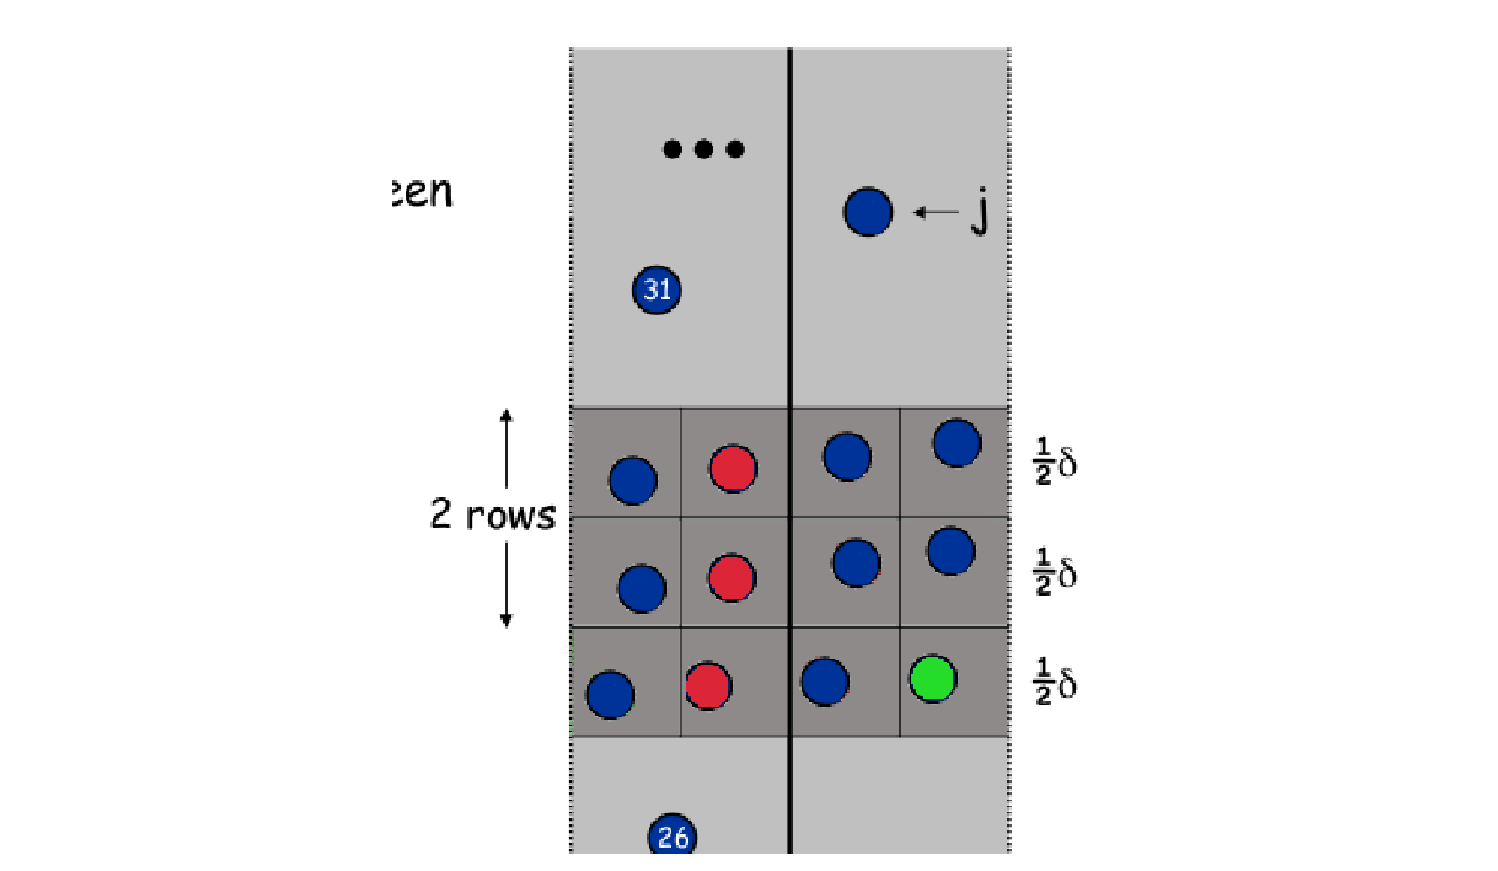
\includegraphics[width=3in] {L5-closestpair-1221delta-strip-7-reason4.eps}
\end{figure}

	对于左边的点,只需要对右边的最多6个点比较即可。我们将条带中的点按照y坐标进行排序,那么只需要找出临近的11个点即可,因为距离它最近的点一定在这11个点里面。
	算法伪代码表示如下:

	{\sc ClosestPair}$( p_i, ..., p_j)$
/*  $p_i,...,p_j$ have already been sorted according to $x$-coordinate; */
\begin{algorithmic}[1]
\IF{ $j-i==1$ }
\STATE return $d(p_{i}, p_{j})$;
\ENDIF
\STATE Use the $x$-coordinate of $p_{\lfloor\frac{i+j}{2}\rfloor}$ to divide $p_i,...,p_j$ into two halves; 
\STATE $\delta_1$ = {\sc ClosestPair}(left half);    \textcolor{red}{ $T(\frac{n}{2})$ } 
\STATE $\delta_2$ = {\sc ClosestPair}(right half);   \textcolor{red}{ $T(\frac{n}{2})$ } 
\STATE $\delta = \min( \delta_1, \delta_2);$
\STATE Sort points within the $2\delta$ strip  by $y$-coordinate; \textcolor{red}{ $O(n \log(n) )$ } 
\STATE Scan points in $y$-order and calculate distance between each point with its next 11 neighbors. Update $\delta$ if finding a distance less than $\delta$;  \textcolor{red}{$O(n)$}
\end{algorithmic}
	Time-complexity: $T(n)=2T(\frac{n}{2}) + O(n \log n) = O(n\log^2(n))$.
	
	
\subsubsection{算法的提升}
	上面算法的合并时间:边界附近的点进行排序需要 $O(n\log n )$ 时间。
	
	如果每一次迭代保持2个序列,一个按照x排序的序列,一个按照y排序的序列。
	像归并排序一样,将预先排序好的2个方向的序列合并起来,实际上只需要$O(n)$的时间。因此时间复杂度是 $T(n)=2T(\frac{n}{2}) + O(n) = O(n\log n)$.
	
	\subsubsection{举例分析:8个点的最近点对}	
	
	
\begin{figure}[H]

	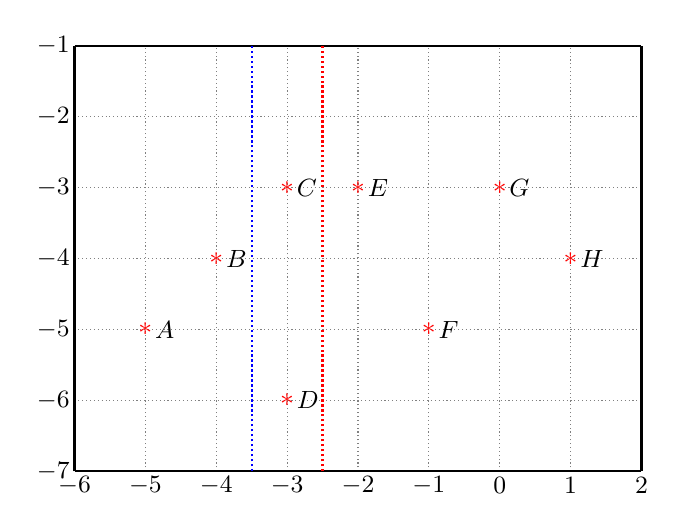
\begin{tikzpicture}[scale=0.9, auto,swap]
%lines
	
	 \foreach \x in { -6, -5, -4, -3, -2, -1, 0, 1, 2}{
	 	\draw[densely dotted, gray] (\x, -7) -- (\x, -1);
		\node at (\x, -7.2) {\small{$\x$}};
	} 	 
	\foreach \y in {-7,  -6, -5, -4, -3, -2, -1}{
	 	\draw[densely dotted, gray] (-6, \y) -- (2, \y);
		\node at (-6.3, \y) {\small{$\y$}};
	} 	
	
        \draw[thick] (-6, -7) -- (2, -7);
        \draw[thick] (-6, -1) -- (2, -1);
        \draw[thick] (-6, -7) -- (-6, -1);
        \draw[thick] (2, -7) -- (2, -1);       
       
%A, B, C
	\foreach \xy/ \name in { {(-5,-5)/A},{(-4,-4)/B},{(-3,-6)/D},{(-3,-3)/C},{(-2,-3)/E},{(-1,-5)/F},{(0,-3)/G},{(1,-4)/H}} {
		\node[red] (\name) at \xy {$*$};
		\node[right] at \xy {\small{$\name$}};
	}       
	
%middle 1 

	        \draw[red, thick, densely dotted] (-2.5, -7) -- (-2.5, -1);       
	        \draw[blue, thick, densely dotted] (-3.5, -7) -- (-3.5, -1);       
%	        \draw[red, thick, densely dotted] (-2.5, -7) -- (-2.5, -1);       
	        

 \end{tikzpicture}		
\end{figure}	


\begin{figure}[H]
	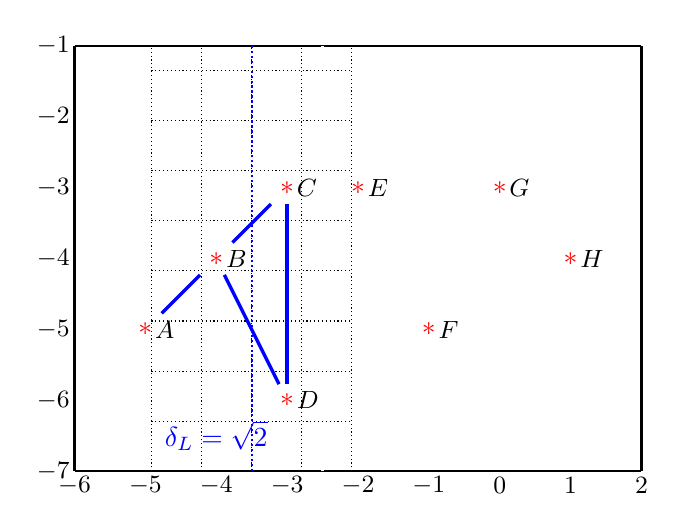
\begin{tikzpicture}[scale=0.9, auto,swap]
%lines
	
	 \foreach \x in { -6, -5, -4, -3, -2, -1, 0, 1, 2}{
%	 	\draw[densely dotted, gray] (\x, -7) -- (\x, -1);
		\node at (\x, -7.2) {\small{$\x$}};
	} 	 
	\foreach \y in {-7,  -6, -5, -4, -3, -2, -1}{
%	 	\draw[densely dotted, gray] (-6, \y) -- (2, \y);
		\node at (-6.3, \y) {\small{$\y$}};
	} 	
	
        \draw[thick] (-6, -7) -- (2, -7);
        \draw[thick] (-6, -1) -- (2, -1);
        \draw[thick] (-6, -7) -- (-6, -1);
        \draw[thick] (2, -7) -- (2, -1);       
       
%A, B, C
	\foreach \xy/ \name in { {(-5,-5)/A},{(-4,-4)/B},{(-3,-6)/D},{(-3,-3)/C},{(-2,-3)/E},{(-1,-5)/F},{(0,-3)/G},{(1,-4)/H}} {
		\node[red] (\name) at \xy {$*$};
		\node[right] at \xy {\small{$\name$}};
	}       
	
%middle 1 

	        \draw[red, thick, densely dotted] (-2.5, -7) -- (-2.5, -1);       
	        
%	        \draw[green, thick, densely dotted] (-0.5, -7) -- (-0.5, -1);       
	        \draw[blue, thick, densely dotted] (-3.5, -7) -- (-3.5, -1);       
%pairs 
	
		\draw[blue, 	very thick] (A) -- (B);
		\draw[blue, 	very thick] (C) -- (D);

		\node[thick, blue] at (-4, -6.5) {$\delta_L=\sqrt{2}$};	
%\delta grids

	
		\draw[white, thick] (-2.5, -7) -- (-2.5, -1);       

		\def\d{1.414 / 2};
		\foreach \i in {-2,...,2}{
			\def\x{-3.5 + \i * \d};
			\draw[black, densely dotted] (\x, -7) -- (\x, -1);
		}
		
		\foreach \i in {1,...,8}{
				\def\y{-7 + \i * \d};
				\draw[black, densely dotted] (-3.5 - 2*\d, \y) -- (-3.5 + 2*\d, \y);	
		}

	        \draw[blue, thick, densely dotted] (-3.5, -7) -- (-3.5, -1);       
			
%		\ifthenelse{ 1.44  <  0 }{
%					\draw[red, 	 thick, densely dotted] (A) -- (B);
%		}{ 
%					\draw[green, 	 thick, densely dotted] (C) -- (B);
%		}
		% B D, B,C 
		

		\draw[blue, 	very thick] (D) -- (B);
		\draw[blue, 	very thick] (C) -- (B);
		
	      \end{tikzpicture}		
	\end{figure}

\begin{footnotesize}
\begin{itemize}
 \item Pair 1: $d(A,B) = \sqrt{2};$
 \item Pair 2: $d(C,D) = 3;$ $\Rightarrow$    $\min = \sqrt{2}; $ Thus, it suffices to calculate:
 \item Pair 3: $d(B,C) = \sqrt{2};$
 \item Pair 4: $d(B,D) = \sqrt{5};$  $\Rightarrow$   $\delta_L = \sqrt{2}$.
\end{itemize}
\end{footnotesize}
	
	
\begin{figure}[H]
	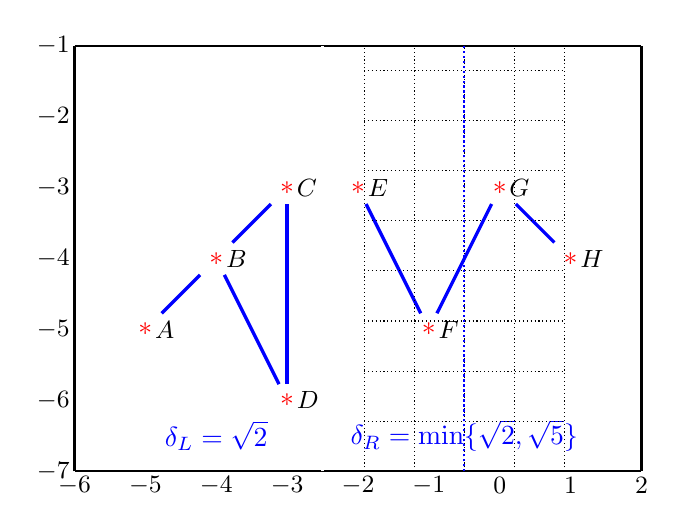
\begin{tikzpicture}[scale=0.9, auto,swap]
%lines
	
	 \foreach \x in { -6, -5, -4, -3, -2, -1, 0, 1, 2}{
%	 	\draw[densely dotted, gray] (\x, -7) -- (\x, -1);
		\node at (\x, -7.2) {\small{$\x$}};
	} 	 
	\foreach \y in {-7,  -6, -5, -4, -3, -2, -1}{
%	 	\draw[densely dotted, gray] (-6, \y) -- (2, \y);
		\node at (-6.3, \y) {\small{$\y$}};
	} 	
	
        \draw[thick] (-6, -7) -- (2, -7);
        \draw[thick] (-6, -1) -- (2, -1);
        \draw[thick] (-6, -7) -- (-6, -1);
        \draw[thick] (2, -7) -- (2, -1);       
       
%A, B, C
	\foreach \xy/ \name in { {(-5,-5)/A},{(-4,-4)/B},{(-3,-6)/D},{(-3,-3)/C},{(-2,-3)/E},{(-1,-5)/F},{(0,-3)/G},{(1,-4)/H}} {
		\node[red] (\name) at \xy {$*$};
		\node[right] at \xy {\small{$\name$}};
	}       
	
%middle 1 
		\node[thick, blue] at (-4, -6.5) {$\delta_L=\sqrt{2}$};	

	        \draw[red, thick, densely dotted] (-2.5, -7) -- (-2.5, -1);       
	        
%	        \draw[green, thick, densely dotted] (-0.5, -7) -- (-0.5, -1);       
	        \draw[blue, thick, densely dotted] (-0.5, -7) -- (-0.5, -1);       

%done
		\draw[blue, 	very thick] (A) -- (B);
		\draw[blue, 	very thick] (B) -- (C);
		\draw[blue, 	very thick] (C) -- (D);
		\draw[blue, 	very thick] (B) -- (D);


%pairs 

		\draw[blue, 	very thick] (E) -- (F);
		\draw[blue, 	very thick] (G) -- (H);

		\node[thick, blue] at (-0.5, -6.5) {$\delta_R=\min\{\sqrt{2}, \sqrt{5}\}$};	
%\delta grids

	
%red line invisible 		
		\draw[white, thick] (-2.5, -7) -- (-2.5, -1);       
%grids
		\def\d{1.414 / 2};
		\foreach \i in {-2,...,2}{
			\def\x{-0.5 + \i * \d};
			\draw[black, densely dotted] (\x, -7) -- (\x, -1);
		}
		
		\foreach \i in {1,...,8}{
				\def\y{-7 + \i * \d};
				\draw[black, densely dotted] (-0.5 - 2*\d, \y) -- (-0.5 + 2*\d, \y);	
		}

	        \draw[blue, thick, densely dotted] (-0.5, -7) -- (-0.5, -1);       
			
%		\ifthenelse{ 1.44  <  0 }{
%					\draw[red, 	 thick, densely dotted] (A) -- (B);
%		}{ 
%					\draw[green, 	 thick, densely dotted] (C) -- (B);
%		}
		% B D, B,C 
		
 
		\draw[blue, 	very thick] (G) -- (F);
		
		
	      \end{tikzpicture}		
	      \end{figure}

\begin{footnotesize}
\begin{itemize}
 \item Pair 5: $d(E,F) = \sqrt{5};$
 \item Pair 6: $d(G,H) = \sqrt{2};$ $\Rightarrow$    $\min = \sqrt{2}; $ Thus, it suffices to calculate:
 \item Pair 7: $d(G,F) = \sqrt{5};$  $\Rightarrow$   $\delta_R = \sqrt{2}$.
\end{itemize}
\end{footnotesize}

\begin{figure}[H]
	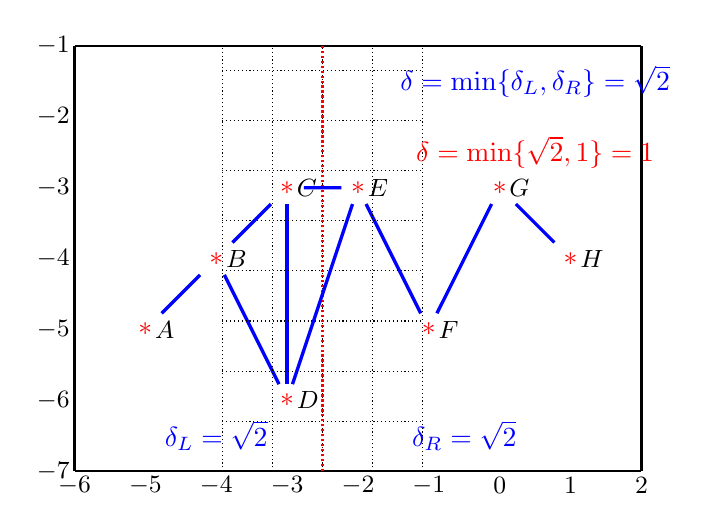
\begin{tikzpicture}[scale=0.9, auto,swap]
%lines
	
	 \foreach \x in { -6, -5, -4, -3, -2, -1, 0, 1, 2}{
%	 	\draw[densely dotted, gray] (\x, -7) -- (\x, -1);
		\node at (\x, -7.2) {\small{$\x$}};
	} 	 
	\foreach \y in {-7,  -6, -5, -4, -3, -2, -1}{
%	 	\draw[densely dotted, gray] (-6, \y) -- (2, \y);
		\node at (-6.3, \y) {\small{$\y$}};
	} 	
	
        \draw[thick] (-6, -7) -- (2, -7);
        \draw[thick] (-6, -1) -- (2, -1);
        \draw[thick] (-6, -7) -- (-6, -1);
        \draw[thick] (2, -7) -- (2, -1);       
       
%A, B, C
	\foreach \xy/ \name in { {(-5,-5)/A},{(-4,-4)/B},{(-3,-6)/D},{(-3,-3)/C},{(-2,-3)/E},{(-1,-5)/F},{(0,-3)/G},{(1,-4)/H}} {
		\node[red] (\name) at \xy {$*$};
		\node[right] at \xy {\small{$\name$}};
	}       

	\node[thick, blue] at (-4, -6.5) {$\delta_L=\sqrt{2}$};	
	\node[thick, blue] at (-0.5, -6.5) {$\delta_R=\sqrt{2}$};	

%middle 1 

	        \draw[red, thick, densely dotted] (-2.5, -7) -- (-2.5, -1);       

%done
		\draw[blue, 	very thick] (A) -- (B);
		\draw[blue, 	very thick] (B) -- (C);
		\draw[blue, 	very thick] (B) -- (D);
		\draw[blue, 	very thick] (C) -- (D);
		\draw[blue, 	very thick] (E) -- (F);
		\draw[blue, 	very thick] (F) -- (G);
		\draw[blue, 	very thick] (G) -- (H);

	        
%	        \draw[green, thick, densely dotted] (-0.5, -7) -- (-0.5, -1);       
%	        \draw[green, thick, densely dotted] (-0.5, -7) -- (-0.5, -1);       
%pairs 

		\node[thick, blue] at (.5, -1.5) {$\delta=\min\{\delta_L, \delta_R\} = \sqrt{2}$};	
%\delta grids

%red line invisible 		
%		\draw[white, thick] (-2.5, -7) -- (-2.5, -1);       
%grids
		\def\d{1.414 / 2};
		\foreach \i in {-2,...,2}{
			\def\x{-2.5 + \i * \d};
			\draw[black, densely dotted] (\x, -7) -- (\x, -1);
		}
		
		\foreach \i in {1,...,8}{
				\def\y{-7 + \i * \d};
				\draw[black, densely dotted] (-2.5 - 2*\d, \y) -- (-2.5 + 2*\d, \y);	
		}
		
	        \draw[white, thick, densely dotted] (-2.5, -7) -- (-2.5, -1);       
	        \draw[red, thick, densely dotted] (-2.5, -7) -- (-2.5, -1);       
			
%		\ifthenelse{ 1.44  <  0 }{
%					\draw[red, 	 thick, densely dotted] (A) -- (B);
%		}{ 
%					\draw[green, 	 thick, densely dotted] (C) -- (B);
%		}
		% B D, B,C 
		

		\draw[blue, 	very thick] (E) -- (D);
		\draw[blue, 	very thick] (E) -- (C);
		
	
		\node[very thick, red] at (.5, -2.5) {$\delta=\min\{\sqrt{2}, 1\} = 1$};	
		
	      \end{tikzpicture}		
	      \end{figure}	


%\begin{figure}
% \includegraphics[height=3in,angle=270] {L5-closestpair-ABCDEFGH-new.eps}
%\end{figure}
\begin{footnotesize}
\begin{itemize}
 \item Pair 8: $d(C,E) = 1;$
 \item Pair 9: $d(D,E) = \sqrt{10};$ $\Rightarrow$   $\delta = 1$.
\end{itemize}
\end{footnotesize}

\begin{figure}[H]
	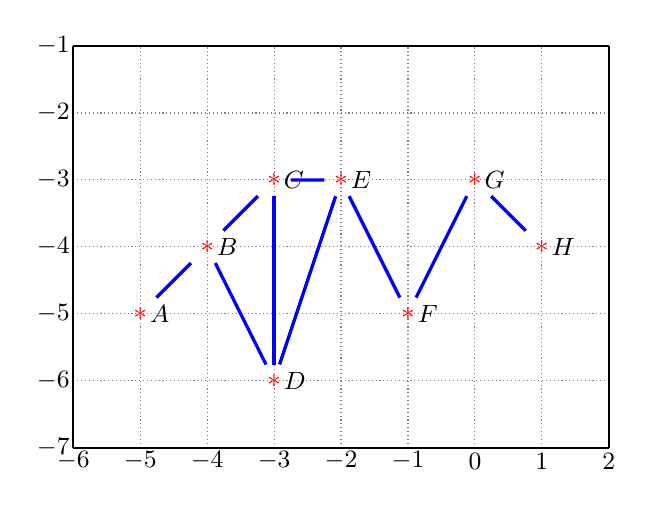
\begin{tikzpicture}[scale=0.85, auto,swap]
%lines
	
	 \foreach \x in { -6, -5, -4, -3, -2, -1, 0, 1, 2}{
	 	\draw[densely dotted, gray] (\x, -7) -- (\x, -1);
		\node at (\x, -7.2) {\small{$\x$}};
	} 	 
	\foreach \y in {-7,  -6, -5, -4, -3, -2, -1}{
	 	\draw[densely dotted, gray] (-6, \y) -- (2, \y);
		\node at (-6.3, \y) {\small{$\y$}};
	} 	
	
        \draw[thick] (-6, -7) -- (2, -7);
        \draw[thick] (-6, -1) -- (2, -1);
        \draw[thick] (-6, -7) -- (-6, -1);
        \draw[thick] (2, -7) -- (2, -1);       
        
       
%A, B, C
	\foreach \xy/ \name in { {(-5,-5)/A},{(-4,-4)/B},{(-3,-6)/D},{(-3,-3)/C},{(-2,-3)/E},{(-1,-5)/F},{(0,-3)/G},{(1,-4)/H}} {
		\node[red] (\name) at \xy {$*$};
		\node[right] at \xy {\small{$\name$}};
	}       
	
%middle 1 

		\draw[blue, 	very thick] (A) -- (B);
		\draw[blue, 	very thick] (B) -- (C);
		\draw[blue, 	very thick] (C) -- (D);

		\draw[blue, 	very thick] (D) -- (B);
		\draw[blue, 	very thick] (C) -- (E);
		\draw[blue, 	very thick] (E) -- (F);

		\draw[blue, 	very thick] (G) -- (H);
		\draw[blue, 	very thick] (G) -- (F);
		\draw[blue, 	very thick] (D) -- (E);


	      \end{tikzpicture}		
	      \end{figure}

\begin{footnotesize}
\begin{itemize}                                                                                                        
\item 
我们只计算了9对点。 剩下的19对是冗余的,原因如下:
\begin{itemize}                                                                                                        
\item 
至少有一个点位于$2\delta$条带之外。
\item 虽然2个点都在 $2\delta$条带内, 但是它们之间的距离超过了2排格子 (格子大小:  $\frac{\delta}{2}\times \frac{\delta}{2}$) 。                                                                                                          \end{itemize}
\end{itemize}
\end{footnotesize}

